% cyclostationary based energy detection
\section{Cyclostationary Detection for multiple Primary Users}
\subsection{System Model}

We consider a cognitive radio system where the spectrum can be occupied by exactly one of two distinct primary signals $\{s_A, s_B\}$ or it could be vacant. Let $H_0$ denote the situation under which the channel is free, $H_1$ denote the hypothesis under which the channel is occupied by signal $s_A$ and $H_2$ denote the hypothesis under which the channel is occupied by signals $s_B$. In this case, we assume $s_A, s_B$ are OFDM signals with same frame structure. The block diagram of the system is illustrated in Figure \ref{pic:1222a0}.

\begin{figure}[!t]
  \centering 
  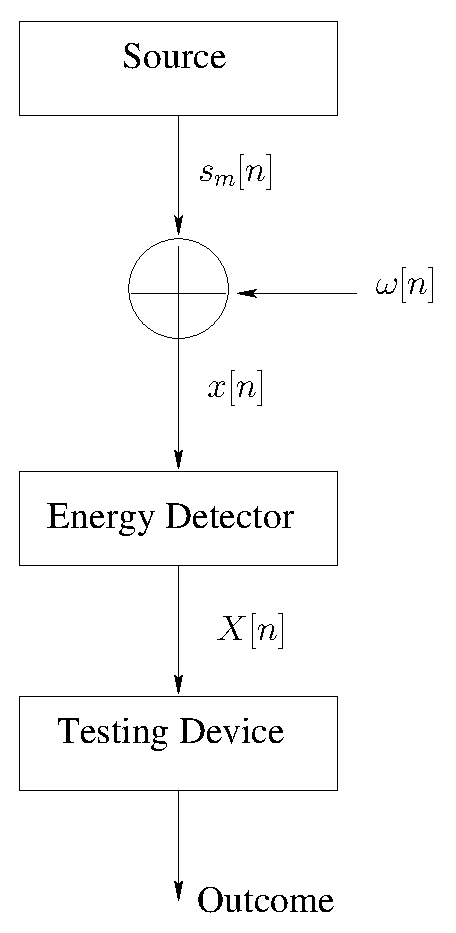
\includegraphics[width=\textwidth]{4/fig1.eps}
  \caption{Block Diagram for  cyclostationary detector.}
  \label{pic:1222a0}
\end{figure}
The measuring device observes $M$ samples of the noise version signals that could present in the channel and output a suitable testing statistics. With this statistics, the testing device employs MENP to determine the status of the channel. The input of measuring device is
\begin{equation}
  \mathbf{x} = \begin{cases}
	\mathbf{n}\;\;\;\;\;\;&\text{when $H_0$ is true}\\
	\mathbf{n}+\mathbf{s}_A\;\;\;\;\;\;&\text{when $H_1$ is true}\\
	\mathbf{n}+\mathbf{s}_B\;\;\;\;\;\;&\text{when $H_2$ is true}\\
  \end{cases}
  \label{equ:1209a1}
\end{equation}
where 
\begin{equation}
  \begin{cases}
	&\mathbf{x} = (x_0, x_1, \cdots, x_{M-1})\\
	&\mathbf{s}_A = (s_{A0}, s_{A1}, \cdots, s_{A(M-1)})\\
	&\mathbf{s}_B = (s_{B0}, s_{B1}, \cdots, s_{B(M-1)})\\
	&\mathbf{n} = (n_{0}, n_{1}, \cdots, n_{M-1})\,.
  \end{cases}
  \label{xssn}
\end{equation}
Assume each OFDM frame contains a CP sequence of length $l_C$ followed by a data sequence of length $l_D$, so the total length of an OFDM frame is $l_0 = l_C+l_D$. In general case, when there are signal transmitting, the receiver is not synchronized to the transmitted signal, i.e. $s_{A0}$ ( or $s_{B0}$) is not the first symbol of an OFDM frame. Let $\tau$ represents the synchronization mismatch. That is, when $\tau = 0$, $s_0$ is the first symbol of an OFDM frame; when $\tau = l_C+l_D -1$, $s_0$ is the last symbol of an OFDM frame. Let $M = Kl_0$, we can see when perfect synchronization the detector would observe $K$ complete  OFDM frames (as it is shown in Figure \ref{pic:1222ext0}); otherwise, the detector would observe $K-1$ complete OFDM frames and $2$ incomplete OFDM frames (as it is shown in Figure \ref{pic:1222a2}). 
\begin{figure}[!t]
  \centering 
  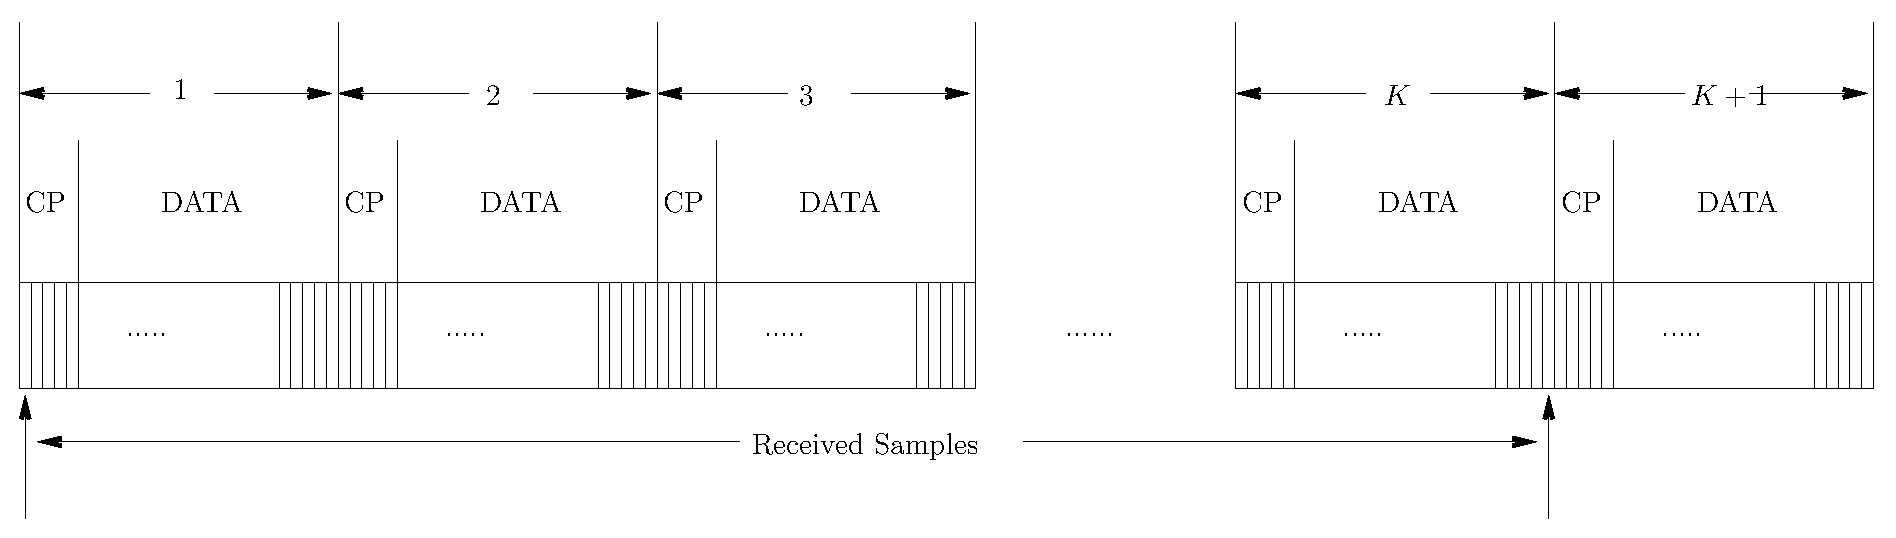
\includegraphics[width=\textwidth]{4/fig2.eps}
  \caption{Received signal for perfect synchronization.}
  \label{pic:1222ext0}
\end{figure}

\begin{figure}[!t]
  \centering 
  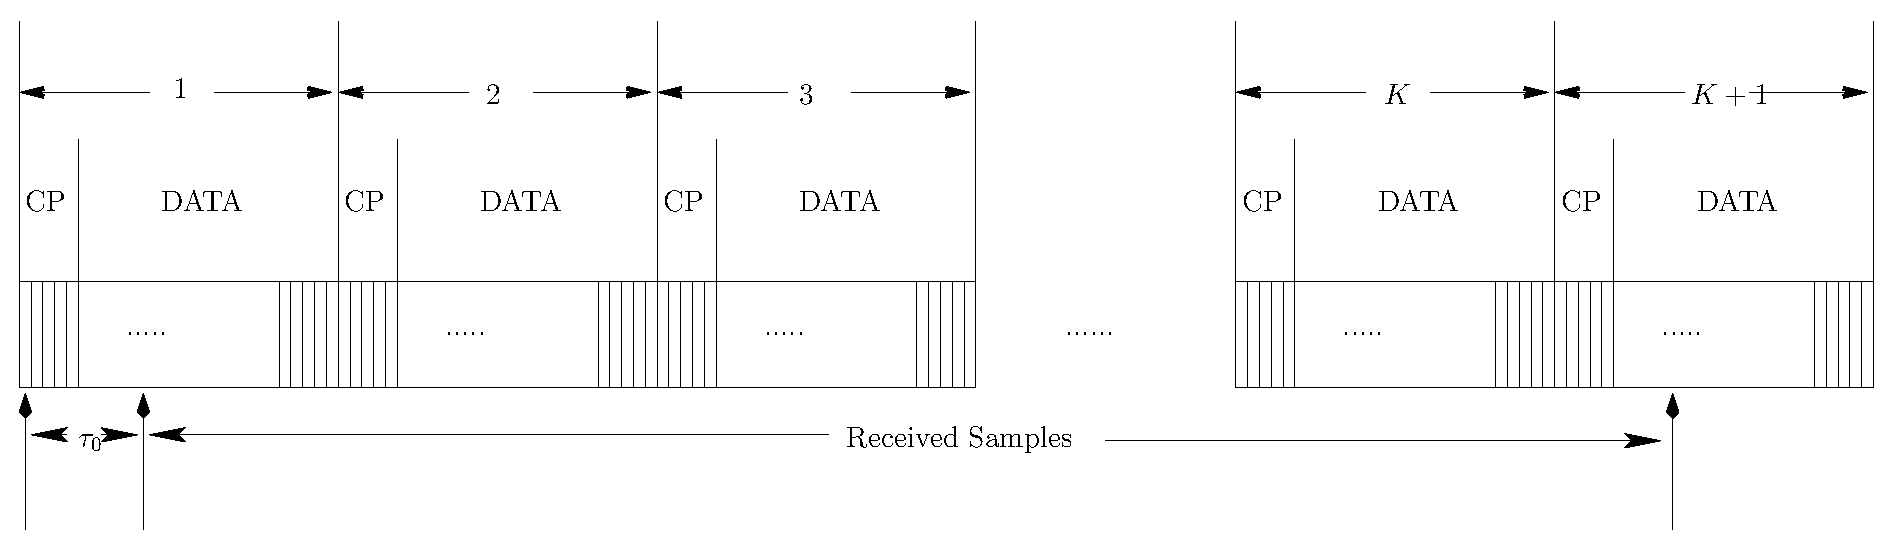
\includegraphics[width=\textwidth]{4/fig3.eps}
  \caption{Received signal for synchronization mismatch $\tau_0$.}
  \label{pic:1222a2}
\end{figure}
Assume $\tau = \tau_0$, let $\Theta_{\tau_0}$ denote the set of subscripts such that if $i \in \Theta_{\tau_0}$,  $s_i$ is a symbol of CP sequence. From Figure \ref{pic:1222ext0} we can see, in the situation of perfect synchronization ( $\tau_0 =0$), when $i \in [Ql_0, Ql_0+l_c-1]$, the associated $s_i$ belongs to CP sequence. 
From Figure \ref{pic:1222a2}, we can see in the situation of imperfect synchronization, $i \in \Theta_{\tau_0}$ only if $i + \tau_0 \in [Ql_0, Ql_0+l_c -1]$ ($Q = 0, 1, \cdots, K-1$). 
Let $\Theta_{\tau_0}^k$ denotes set $\Theta_{\tau_0}$ subtract set $\{k\}$ ($k$ is also a subscript), i.e.
\begin{equation}
  \{i\in \Theta_{\tau_0}^k| i + \tau_0 \in [Ql_0, Ql_0+l_c -1] (Q = 0, 1, \cdots, K-1)\;\;\;\; \text{and}\;\;\;\; i\neq k\}
  \label{definitionof}
\end{equation}

Like in  \cite{axell2011optimal}, we make following assumptions about the noise and signal: (1) all noise samples are i.i.d. mean zero circularly symmetric complex Gaussian (CSCG) with variance $\sigma_n^2$; (2) under hypothesis $H_1$ the transmitted signal symbols in the data sequence are i.i.d. zero mean CSCG with variance $\sigma_{s_A}^2$ (or $\sigma_{s_B}^2$ under hypothesis $H_2$); (3) if $s_i$ is a sample in CP sequence, then we have $s_i = s_{i+l_D}$. 

The CP structure could introduce strong cyclostationarity to the transmitted OFDM signals ($s_A$ or $s_B$) \cite{lunden2010robust}. 
Let $r_i=x_ix_j^\ast$ ($j=i+l_D$), \cite{lunden2007spectrum} shows $r_i$ exhibit cyclic property at frequency $\alpha = \frac{Q}{l_0}$ ($Q = \pm1, \pm2, \cdots$). In this case, we consider a single cyclic detector at frequency $\alpha = \frac{1}{l_0}$. 
Let $\mathbf{r}$ denote the vector of $r_i$, since the length of vector $\mathbf{x}$ is $M$, the length of $\mathbf{r}$ is $M - l_D$. For simple representation, let $N = M - l_D$.
Like in most related literature reviews (c.f. \cite{lunden2010robust} \cite{dandawate1994statistical}), the cyclic-covariance estimator for frequency $\alpha$ can be written as
\begin{equation}
  \hat{R}(l_D, \alpha) = \frac{1}{N}\sum_{i=0}^{N-1} r_ib_i\,.
  \label{cyclicR}
\end{equation}
where $b_i = \exp(-j2\pi\alpha i)$. 
The output of the measuring device is the real and imaginary part of the cyclic covariance estimator, i.e. 
\begin{equation}
  Y = \begin{bmatrix}
	R \\
	I
  \end{bmatrix}\,,
  \label{cyclic_cov}
\end{equation}
where 
\[
  R = \Re(\hat{R}(l_D, \alpha))
\]
and 
\[
  I = \Im(\hat{R}(l_D, \alpha))\,.
\]
By observing $y$, a realization  of $Y$, the testing device determines the status of the channel.
According to \cite{lunden2010robust}, $\hat{R}(l_D, \alpha)$ subjects to normal distribution for a large $K$, so $Y$ has the two-dimensional Gaussian distribution \cite{goodman1963statistical}.
Let $\bar{c}$ and $\tilde{c}$ denote the real and imaginary parts of a complex number $c$ respectively. Then, $b_i = \bar{b}_i + j\tilde{b}_i$  and $r_i = \bar{r}_i + j\tilde{r}_i$. 

The moment function of $\bar{r}_i, \tilde{r}_i$ are derived in \cite{axell2011optimal} and summarized in Table \ref{Table1} on page \pageref{Table1}.

% Please add the following required packages to your document preamble:
% \usepackage{multirow}
\begin{table}[h]
\centering
  \begin{tabular}{|c|c|c|c|c|c|}
	\hline
	\multirow{2}{*}{}           & \multirow{2}{*}{$H_0$} & \multicolumn{2}{c|}{$H_1$}                                                               & \multicolumn{2}{c|}{$H_2$}                                                               \\ \cline{3-6} 
	&                        & $i \in \Theta_{\tau_0}$                                                   & $i\notin \Theta_{\tau_0}$                          & $i\in \Theta_{\tau_0}$                                                   & $i\notin \Theta_{\tau_0}$                          \\ \hline
	$E[\bar{r}_i]$              & $0$                    & $2\sigma_{s_A}^2$                                       & $0$                            & $2\sigma_{s_B}^2$                                                         & $0$                            \\ \hline
	$E[\tilde{r}_i]$            & $0$                    & $0$                                                     & $0$                            & $0$                                                     & $0$                            \\ \hline
	$E[\bar{r}_i^2]$            & $2\sigma_n^4$          & $8\sigma_{s_A}^4+4\sigma_{s_A}^2\sigma_n^2+2\sigma_n^4$ & $2(\sigma_n^2+\sigma_{s_A}^2)^2$ & $8\sigma_{s_B}^4+4\sigma_{s_B}^2\sigma_n^2+2\sigma_n^4$ & $2(\sigma_n^2+\sigma_{s_B}^2)^2$ \\ \hline
	$E[\tilde{r}_i^2]$          & $2\sigma_n^4$          & $4\sigma_{s_A}^2\sigma_n^2+2\sigma_n^4$                 & $2(\sigma_n^2+\sigma_{s_A}^2)^2$ & $4\sigma_{s_B}^2\sigma_n^2+2\sigma_n^4$                 & $2(\sigma_n^2+\sigma_{s_B}^2)^2$ \\ \hline
	$E[\bar{r}_i\tilde{r}_i]$   & $0$                    & $0$                                                     & $0$                            & $0$                                                     & $0$                            \\ \hline
  \end{tabular}
  \caption{Moment function of $r_i$}
  \label{Table1}
\end{table}

Next we compute $E[\bar{r}_i\bar{r}_k]$, $E[\bar{r}_i\tilde{r}_k]$ and $E[\tilde{r}_i\tilde{r}_k]$ when $i \neq k$ under hypothesis $H_1$. For easy presentation, let $j = i+l_D$ and $l=k+l_D$.
 The expression of $r_i$ can be written as
\begin{equation}
  \begin{split}
    r_i = &(s_i+n_i)(s_j + n_j)^\ast\\
    = &(\bar{s}_i+j\tilde{s}_i + \bar{n}_i+j\tilde{n}_i)(\bar{s}_j-j\tilde{s}_j + \bar{n}_j-j\tilde{n}_j)\\
    = &\bar{s}_i\bar{s}_j + \bar{s}_i\bar{n}_j +\tilde{s}_i\tilde{s}_j+\tilde{s}_i\tilde{n}_j + \bar{n}_i\bar{s}_j+\bar{n}_i\bar{n}_j+\tilde{n}_i\tilde{s}_j+\tilde{n}_i\tilde{n}_j\\
    + &j\left( \tilde{s}_i\bar{s}_j + \tilde{s}_i\bar{n}_j + \tilde{n}_i\bar{s}_j + \tilde{n}_i\bar{n}_j - \bar{s}_i\tilde{s}_j - \bar{s}_i\tilde{n}_j - \bar{n}_i\tilde{s}_j - \bar{n}_i\tilde{n}_j \right)
  \end{split}
\end{equation}
thus we have 
\begin{equation}
  \begin{cases}
    \bar{r}_i = \bar{s}_i\bar{s}_j + \bar{s}_i\bar{n}_j +\tilde{s}_i\tilde{s}_j+\tilde{s}_i\tilde{n}_j + \bar{n}_i\bar{s}_j+\bar{n}_i\bar{n}_j+\tilde{n}_i\tilde{s}_j+\tilde{n}_i\tilde{n}_j\\
    \tilde{r}_i = \tilde{s}_i\bar{s}_j + \tilde{s}_i\bar{n}_j + \tilde{n}_i\bar{s}_j + \tilde{n}_i\bar{n}_j - \bar{s}_i\tilde{s}_j - \bar{s}_i\tilde{n}_j - \bar{n}_i\tilde{s}_j - \bar{n}_i\tilde{n}_j\,.
  \end{cases}
  \label{RrIr}
\end{equation}

\begin{equation}
  \begin{split}
    E[\bar{r}_i\bar{r}_k] = &E[(\bar{s}_i\bar{s}_j + \bar{s}_i\bar{n}_j +\tilde{s}_i\tilde{s}_j+\tilde{s}_i\tilde{n}_j + \bar{n}_i\bar{s}_j+\bar{n}_i\bar{n}_j+\tilde{n}_i\tilde{s}_j+\tilde{n}_i\tilde{n}_j)\\
    &(\bar{s}_k\bar{s}_l + \bar{s}_k\bar{n}_l +\tilde{s}_k\tilde{s}_l+\tilde{s}_k\tilde{n}_l + \bar{n}_k\bar{s}_l+\bar{n}_k\bar{n}_l+\tilde{n}_k\tilde{s}_l+\tilde{n}_k\tilde{n}_l)]\\
    = &E[\bar{s}_j\bar{s}_k\bar{s}_i\bar{s}_l]+E[\bar{s}_j\bar{s}_k\bar{s}_i\bar{n}_l]+E[\bar{s}_j\tilde{s}_k\bar{s}_i\tilde{s}_l]+E[\bar{s}_j\tilde{s}_k\bar{s}_i\tilde{n}_l]+E[\bar{s}_j\bar{n}_k\bar{s}_i\bar{s}_l]\\
&+E[\bar{s}_j\bar{n}_k\bar{s}_i\bar{n}_l]+E[\bar{s}_j\tilde{n}_k\bar{s}_i\tilde{s}_l]+E[\bar{s}_j\tilde{n}_k\bar{s}_i\tilde{n}_l]+E[\bar{n}_j\bar{s}_i\bar{s}_l\bar{s}_k]+E[\bar{n}_j\bar{s}_i\bar{n}_l\bar{s}_k]\\
&+E[\tilde{s}_k\bar{n}_j\bar{s}_i\tilde{s}_l]+E[\tilde{s}_k\bar{n}_j\bar{s}_i\tilde{n}_l]+E[\bar{n}_j\bar{n}_k\bar{s}_i\bar{s}_l]+E[\bar{n}_j\bar{n}_k\bar{s}_i\bar{n}_l]+E[\bar{n}_j\tilde{n}_k\bar{s}_i\tilde{s}_l]\\
&+E[\bar{n}_j\tilde{n}_k\bar{s}_i\tilde{n}_l]+E[\tilde{s}_j\tilde{s}_i\bar{s}_l\bar{s}_k]+E[\tilde{s}_j\tilde{s}_i\bar{n}_l\bar{s}_k]+E[\tilde{s}_k\tilde{s}_j\tilde{s}_i\tilde{s}_l]+E[\tilde{s}_k\tilde{s}_j\tilde{s}_i\tilde{n}_l]\\
&+E[\tilde{s}_j\tilde{s}_i\bar{n}_k\bar{s}_l]+E[\tilde{s}_j\tilde{s}_i\bar{n}_k\bar{n}_l]+E[\tilde{s}_j\tilde{s}_i\tilde{n}_k\tilde{s}_l]+E[\tilde{s}_j\tilde{s}_i\tilde{n}_k\tilde{n}_l]+E[\bar{s}_k\tilde{s}_i\tilde{n}_j\bar{s}_l]\\
&+E[\bar{s}_k\tilde{s}_i\tilde{n}_j\bar{n}_l]+E[\tilde{s}_k\tilde{s}_i\tilde{n}_j\tilde{s}_l]+E[\tilde{s}_k\tilde{s}_i\tilde{n}_l\tilde{n}_j]+E[\tilde{s}_i\bar{n}_k\tilde{n}_j\bar{s}_l]+E[\tilde{s}_i\bar{n}_k\tilde{n}_j\bar{n}_l]\\
&+E[\tilde{s}_i\tilde{n}_k\tilde{n}_j\tilde{s}_l]+E[\tilde{s}_i\tilde{n}_k\tilde{n}_l\tilde{n}_j]+E[\bar{n}_i\bar{s}_j\bar{s}_l\bar{s}_k]+E[\bar{n}_i\bar{s}_j\bar{n}_l\bar{s}_k]+E[\bar{n}_i\bar{s}_j\tilde{s}_k\tilde{s}_l]\\
&+E[\bar{n}_i\bar{s}_j\tilde{n}_l\tilde{s}_k]+E[\bar{n}_i\bar{s}_j\bar{n}_k\bar{s}_l]+E[\bar{n}_i\bar{s}_j\bar{n}_k\bar{n}_l]+E[\bar{n}_i\bar{s}_j\tilde{n}_k\tilde{s}_l]+E[\bar{n}_i\bar{s}_j\tilde{n}_k\tilde{n}_l]\\
&+E[\bar{n}_i\bar{s}_k\bar{n}_j\bar{s}_l]+E[\bar{n}_i\bar{s}_k\bar{n}_j\bar{n}_l]+E[\bar{n}_i\tilde{s}_k\bar{n}_j\tilde{s}_l]+E[\bar{n}_i\tilde{s}_k\bar{n}_j\tilde{n}_l]+E[\bar{n}_i\bar{n}_k\bar{n}_j\bar{s}_l]\\
&+E[\bar{n}_i\bar{n}_k\bar{n}_j\bar{n}_l]+E[\bar{n}_i\tilde{n}_k\bar{n}_j\tilde{s}_l]+E[\bar{n}_i\tilde{n}_k\bar{n}_j\tilde{n}_l]+E[\tilde{n}_i\bar{s}_k\bar{s}_l\tilde{s}_j]+E[\tilde{n}_i\bar{n}_l\bar{s}_k\tilde{s}_j]\\
&+E[\tilde{s}_k\tilde{n}_i\tilde{s}_l\tilde{s}_j]+E[\tilde{s}_k\tilde{n}_i\tilde{n}_l\tilde{s}_j]+E[\tilde{n}_i\bar{n}_k\bar{s}_l\tilde{s}_j]+E[\tilde{n}_i\bar{n}_k\bar{n}_l\tilde{s}_j]+E[\tilde{s}_l\tilde{n}_i\tilde{n}_k\tilde{s}_j]\\
&+E[\tilde{n}_i\tilde{n}_k\tilde{n}_l\tilde{s}_j]+E[\tilde{n}_i\tilde{n}_j\bar{s}_l\bar{s}_k]+E[\tilde{n}_i\tilde{n}_j\bar{n}_l\bar{s}_k]+E[\tilde{s}_k\tilde{n}_i\tilde{n}_j\tilde{s}_l]+E[\tilde{s}_k\tilde{n}_i\tilde{n}_j\tilde{n}_l]\\
&+E[\tilde{n}_i\tilde{n}_j\bar{n}_k\bar{s}_l]+E[\tilde{n}_i\tilde{n}_j\bar{n}_k\bar{n}_l]+E[\tilde{n}_i\tilde{n}_j\tilde{n}_k\tilde{s}_l]+E[\tilde{n}_i\tilde{n}_j\tilde{n}_k\tilde{n}_l]
  \end{split}
  \label{Erij}
\end{equation}
Since noise samples are governed by i.i.d Gaussian distribution with zero mean and they are independent with signals, items in \eqref{Erij} containing noise samples would have zero value, e.g. $E[\bar{s}_j\bar{s}_k\bar{s}_i\bar{n}_l] = E[\bar{s}_j\bar{s}_k\bar{s}_i]E[\bar{n}_l] = 0$. Eliminate zero value items in equation \eqref{Erij}:
\begin{equation}
  E[\bar{r}_i\bar{r}_k] = E[\bar{s}_i\bar{s}_j\bar{s}_k\bar{s}_l] + E[\bar{s}_i\bar{s}_j\tilde{s}_k\tilde{s}_l] + E[\tilde{s}_i\tilde{s}_j\bar{s}_k\bar{s}_l] + E[\tilde{s}_i\tilde{s}_j\tilde{s}_k\tilde{s}_l]
  \label{equ:Erirk}
\end{equation} 

Without losing generality, we assume $i < k$. Consider the situation when $k \notin \Theta_{\tau_0}$, in such case $s_k$ is a symbol in data sequence so $s_k$ and $s_{k+l_D}$ are independent, i.e. $s_k$ and $s_l$ are independent. Furether more, it is easy to see $s_l$ is also independent with $s_i$ and $s_j$. Hence \eqref{equ:Erirk} can be written as
\begin{equation}
  \begin{split}
  E[\bar{r}_i\bar{r}_k] = &E[\bar{s}_i\bar{s}_j\bar{s}_k]E[\bar{s}_l] + E[\bar{s}_i\bar{s}_j\tilde{s}_k]E[\tilde{s}_l] + E[\tilde{s}_i\tilde{s}_j\bar{s}_k]E[\bar{s}_l] + E[\tilde{s}_i\tilde{s}_j\tilde{s}_k]E[\tilde{s}_l]\\
  = &0\,.
\end{split}
  \label{equ:Erirksitu1}
\end{equation} 
Similarly it can be proved when $i \notin \Theta_{\tau_0}$, we have $E[\bar{r}_i\bar{r}_k] =0$. Now consider the situation when $i, k \in \Theta_{\tau_0}$. In such case, we have 
\begin{equation}
  \begin{cases}
    s_i = s_j\\
    s_k = s_l
  \end{cases}
\end{equation}
and \eqref{equ:Erirk} can be written in form of
\begin{equation}
  \begin{split}
    E[\bar{r}_i\bar{r}_k] &= E[\bar{s}_i^2\bar{s}_k^2] + E[\bar{s}_i^2\tilde{s}_k^2]  +E[\tilde{s}_i^2\bar{s}_k^2] + E[\tilde{s}_i^2\tilde{s}_k^2] \\
    &= E[\bar{s}_i^2]E[\bar{s}_k^2] + E[\bar{s}_i^2]E[\tilde{s}_k^2]  +E[\tilde{s}_i^2]E[\bar{s}_k^2] + E[\tilde{s}_i^2]E[\tilde{s}_k^2] \\
    &= 4\sigma_{s_A}^4\,.
  \end{split}
  \label{Eririsitu2}
\end{equation}

From above discussion, the value of $E[\bar{r}_i\bar{r}_k]$  ($i \neq k$) can be summarized as
\begin{equation}
  E[\bar{r}_i\bar{r}_k] =  \begin{cases}
    4\sigma_{s_A}^4 \;\;\;\;&i, k \in \Theta_{\tau_0}\\
    0\;\;\;\;&\text{Otherwise}
  \end{cases}
  \label{Er_ir_j}
\end{equation}

Next consider $E[\bar{r}_i\tilde{r}_j]$, which can be written as
\begin{equation}
  \begin{split}
E[\bar{r}_i\tilde{r}_j] = &E[(\bar{s}_i\bar{s}_j + \bar{s}_i\bar{n}_j +\tilde{s}_i\tilde{s}_j+\tilde{n}_i\tilde{n}_j + \bar{n}_i\bar{s}_j+\bar{n}_i\bar{n}_j+\tilde{n}_i\tilde{s}_j+\tilde{n}_i\tilde{n}_j)\\
              &(\tilde{s}_k\bar{s}_l + \tilde{s}_k\bar{n}_l + \tilde{n}_k\bar{s}_l + \tilde{n}_k\bar{n}_l - \bar{s}_k\tilde{s}_l - \bar{s}_k\tilde{n}_l - \bar{n}_k\tilde{s}_l - \bar{n}_k\tilde{n}_l)]\,.
%              = &E[\bar{s}_j\tilde{s}_k\bar{s}_i\bar{s}_l]+E[\bar{s}_j\tilde{s}_k\bar{s}_i\bar{n}_l]+E[\bar{s}_j\tilde{n}_k\bar{s}_i\bar{s}_l]+E[\bar{s}_j\tilde{n}_k\bar{s}_i\bar{n}_l]-E[\bar{s}_j\bar{s}_k\bar{s}_i\tilde{s}_l]\\
%&-E[\bar{s}_j\bar{s}_k\bar{s}_i\tilde{n}_l]-E[\bar{s}_j\bar{n}_k\bar{s}_i\tilde{s}_l]-E[\bar{s}_j\bar{n}_k\bar{s}_i\tilde{n}_l]+E[\tilde{s}_k\bar{n}_j\bar{s}_i\bar{s}_l]+E[\tilde{s}_k\bar{n}_j\bar{s}_i\bar{n}_l]\\
%&+E[\bar{n}_j\tilde{n}_k\bar{s}_i\bar{s}_l]+E[\bar{n}_j\tilde{n}_k\bar{s}_i\bar{n}_l]-E[\tilde{s}_l\bar{n}_j\bar{s}_i\bar{s}_k]-E[\bar{n}_j\bar{s}_i\tilde{n}_l\bar{s}_k]-E[\bar{n}_j\bar{n}_k\bar{s}_i\tilde{s}_l]\\
%&-E[\bar{n}_j\bar{n}_k\bar{s}_i\tilde{n}_l]+E[\tilde{s}_k\tilde{s}_j\tilde{s}_i\bar{s}_l]+E[\tilde{s}_k\tilde{s}_j\tilde{s}_i\bar{n}_l]+E[\tilde{s}_j\tilde{s}_i\tilde{n}_k\bar{s}_l]+E[\tilde{s}_j\tilde{s}_i\tilde{n}_k\bar{n}_l]\\
%&-E[\tilde{s}_j\tilde{s}_i\tilde{s}_l\bar{s}_k]-E[\tilde{s}_j\tilde{s}_i\tilde{n}_l\bar{s}_k]-E[\tilde{s}_j\tilde{s}_i\bar{n}_k\tilde{s}_l]-E[\tilde{s}_j\tilde{s}_i\tilde{n}_l\bar{n}_k]+E[\tilde{s}_k\tilde{n}_i\tilde{n}_j\bar{s}_l]\\
%&+E[\tilde{s}_k\tilde{n}_i\tilde{n}_j\bar{n}_l]+E[\tilde{n}_i\tilde{n}_j\tilde{n}_k\bar{s}_l]+E[\tilde{n}_i\tilde{n}_j\tilde{n}_k\bar{n}_l]-E[\tilde{n}_i\tilde{n}_j\tilde{s}_l\bar{s}_k]-E[\tilde{n}_i\tilde{n}_j\tilde{n}_l\bar{s}_k]\\
%&-E[\tilde{n}_i\tilde{n}_j\bar{n}_k\tilde{s}_l]-E[\tilde{n}_i\tilde{n}_j\tilde{n}_l\bar{n}_k]+E[\bar{n}_i\bar{s}_j\bar{s}_l\tilde{s}_k]+E[\bar{n}_i\bar{s}_j\bar{n}_l\tilde{s}_k]+E[\bar{n}_i\bar{s}_j\tilde{n}_k\bar{s}_l]\\
%&+E[\bar{n}_i\bar{s}_j\tilde{n}_k\bar{n}_l]-E[\bar{n}_i\bar{s}_j\tilde{s}_l\bar{s}_k]-E[\bar{n}_i\bar{s}_j\tilde{n}_l\bar{s}_k]-E[\bar{n}_i\bar{s}_j\bar{n}_k\tilde{s}_l]-E[\bar{n}_i\bar{s}_j\bar{n}_k\tilde{n}_l]\\
%&+E[\bar{n}_i\tilde{s}_k\bar{n}_j\bar{s}_l]+E[\bar{n}_i\tilde{s}_k\bar{n}_j\bar{n}_l]+E[\bar{n}_i\tilde{n}_k\bar{n}_j\bar{s}_l]+E[\bar{n}_i\tilde{n}_k\bar{n}_j\bar{n}_l]-E[\bar{n}_i\bar{s}_k\bar{n}_j\tilde{s}_l]\\
%&-E[\bar{n}_i\bar{s}_k\bar{n}_j\tilde{n}_l]-E[\bar{n}_i\bar{n}_k\bar{n}_j\tilde{s}_l]-E[\bar{n}_i\bar{n}_k\bar{n}_j\tilde{n}_l]+E[\tilde{s}_k\tilde{n}_i\bar{s}_l\tilde{s}_j]+E[\tilde{s}_k\tilde{n}_i\bar{n}_l\tilde{s}_j]\\
%&+E[\tilde{n}_i\tilde{n}_k\bar{s}_l\tilde{s}_j]+E[\tilde{n}_i\tilde{n}_k\bar{n}_l\tilde{s}_j]-E[\tilde{n}_i\tilde{s}_l\bar{s}_k\tilde{s}_j]-E[\tilde{n}_i\tilde{n}_l\bar{s}_k\tilde{s}_j]-E[\tilde{n}_i\bar{n}_k\tilde{s}_l\tilde{s}_j]\\
%&-E[\tilde{n}_i\bar{n}_k\tilde{n}_l\tilde{s}_j]+E[\tilde{s}_k\tilde{n}_i\tilde{n}_j\bar{s}_l]+E[\tilde{s}_k\tilde{n}_i\tilde{n}_j\bar{n}_l]+E[\tilde{n}_i\tilde{n}_j\tilde{n}_k\bar{s}_l]+E[\tilde{n}_i\tilde{n}_j\tilde{n}_k\bar{n}_l]\\
%&-E[\tilde{n}_i\tilde{n}_j\tilde{s}_l\bar{s}_k]-E[\tilde{n}_i\tilde{n}_j\tilde{n}_l\bar{s}_k]-E[\tilde{n}_i\tilde{n}_j\bar{n}_k\tilde{s}_l]-E[\tilde{n}_i\tilde{n}_j\tilde{n}_l\bar{n}_k]
\end{split}
\label{Eriiiirk}
\end{equation}
expand \eqref{Eriiiirk} and eliminate zero value items (items including noise samples), we have 
 \begin{equation}
   E[\bar{r}_i\tilde{r}_k] = E[\bar{s}_j\tilde{s}_k\bar{s}_i\bar{s}_l] -  E[\bar{s}_j\bar{s}_k\bar{s}_i\tilde{s}_l] + E[\tilde{s}_j\tilde{s}_k\tilde{s}_i\bar{s}_l] - E[\tilde{s}_j\bar{s}_k\tilde{s}_i\tilde{s}_l]\,.
   \label{equ:1213a}
\end{equation}
Since the real and imaginary part of transmitted OFDM signals are independent and $E[\bar{s}_m] = E[\tilde{s}_m] = 0$ ($m = 0, 1, \cdots, N$), \eqref{equ:1213a} can be written as
\begin{equation}
  \begin{split}
  E[\bar{r}_i\tilde{r}_k] &= E[\tilde{s}_k]E[\bar{s}_i\bar{s}_j\bar{s}_l]  - E[\tilde{s}_l]E[\bar{s}_i\bar{s}_j\bar{s}_k] + E[\bar{s}_l]E[\tilde{s}_i\tilde{s}_j\tilde{s}_k] -  E[\bar{s}_k]E[\tilde{s}_i\tilde{s}_j\tilde{s}_l]\\
  &= 0
\end{split}
  \label{equ:1215m}
\end{equation}
thus we can see $E[\bar{r}_i\tilde{r}_k] = 0$  when $i \neq k $.  

Next consider $E[\tilde{r}_i\tilde{r}_k]$, which can be written as
\begin{equation}
  \begin{split}
    E[\tilde{r}_i\tilde{r}_k] = &E[(\tilde{s}_i\bar{s}_j + \tilde{s}_i\bar{n}_j + \tilde{n}_i\bar{s}_j + \tilde{n}_i\bar{n}_j - \bar{s}_i\tilde{s}_j - \bar{s}_i\tilde{n}_j - \bar{n}_i\tilde{s}_j - \bar{n}_i\tilde{n}_j)\\
    &(\tilde{s}_k\bar{s}_l + \tilde{s}_k\bar{n}_l + \tilde{n}_k\bar{s}_l + \tilde{n}_k\bar{n}_l - \bar{s}_k\tilde{s}_l - \bar{s}_k\tilde{n}_l - \bar{n}_k\tilde{s}_l - \bar{n}_k\tilde{n}_l)]
%    = &E[\bar{s}_j\tilde{s}_k\tilde{s}_i\bar{s}_l]+E[\bar{s}_j\tilde{s}_k\tilde{s}_i\bar{n}_l]+E[\bar{s}_j\tilde{s}_i\tilde{n}_k\bar{s}_l]+E[\bar{s}_j\tilde{s}_i\tilde{n}_k\bar{n}_l]-E[\bar{s}_j\bar{s}_k\tilde{s}_i\tilde{s}_l]\\
%&-E[\bar{s}_j\bar{s}_k\tilde{s}_i\tilde{n}_l]-E[\bar{s}_j\tilde{s}_i\bar{n}_k\tilde{s}_l]-E[\bar{s}_j\tilde{s}_i\tilde{n}_l\bar{n}_k]+E[\tilde{s}_k\tilde{s}_i\bar{n}_j\bar{s}_l]+E[\tilde{s}_k\tilde{s}_i\bar{n}_j\bar{n}_l]\\
%&+E[\tilde{n}_k\tilde{s}_i\bar{n}_j\bar{s}_l]+E[\tilde{n}_k\tilde{s}_i\bar{n}_j\bar{n}_l]-E[\bar{s}_k\tilde{s}_i\bar{n}_j\tilde{s}_l]-E[\bar{s}_k\tilde{s}_i\bar{n}_j\tilde{n}_l]-E[\tilde{s}_i\bar{n}_j\bar{n}_k\tilde{s}_l]\\
%&-E[\tilde{s}_i\bar{n}_j\tilde{n}_l\bar{n}_k]+E[\bar{s}_j\tilde{n}_i\bar{s}_l\tilde{s}_k]+E[\bar{s}_j\tilde{n}_i\bar{n}_l\tilde{s}_k]+E[\bar{s}_j\tilde{n}_i\tilde{n}_k\bar{s}_l]+E[\bar{s}_j\tilde{n}_i\tilde{n}_k\bar{n}_l]\\
%&-E[\bar{s}_j\tilde{n}_i\tilde{s}_l\bar{s}_k]-E[\bar{s}_j\tilde{n}_i\tilde{n}_l\bar{s}_k]-E[\bar{s}_j\tilde{n}_i\bar{n}_k\tilde{s}_l]-E[\bar{s}_j\tilde{n}_i\bar{n}_k\tilde{n}_l]+E[\tilde{s}_k\tilde{n}_i\bar{n}_j\bar{s}_l]\\
%&+E[\tilde{s}_k\tilde{n}_i\bar{n}_j\bar{n}_l]+E[\tilde{n}_i\tilde{n}_k\bar{n}_j\bar{s}_l]+E[\tilde{n}_i\tilde{n}_k\bar{n}_j\bar{n}_l]-E[\tilde{s}_l\tilde{n}_i\bar{n}_j\bar{s}_k]-E[\tilde{n}_i\bar{n}_j\tilde{n}_l\bar{s}_k]\\
%&-E[\tilde{n}_i\bar{n}_k\bar{n}_j\tilde{s}_l]-E[\tilde{n}_i\bar{n}_k\bar{n}_j\tilde{n}_l]-E[\tilde{s}_k\tilde{s}_j\bar{s}_i\bar{s}_l]-E[\tilde{s}_k\tilde{s}_j\bar{s}_i\bar{n}_l]-E[\tilde{s}_j\tilde{n}_k\bar{s}_i\bar{s}_l]\\
%&-E[\tilde{s}_j\tilde{n}_k\bar{s}_i\bar{n}_l]+E[\tilde{s}_l\tilde{s}_j\bar{s}_i\bar{s}_k]+E[\tilde{s}_j\bar{s}_i\tilde{n}_l\bar{s}_k]+E[\tilde{s}_j\bar{n}_k\bar{s}_i\tilde{s}_l]+E[\tilde{s}_j\bar{n}_k\bar{s}_i\tilde{n}_l]\\
%&-E[\tilde{s}_k\tilde{n}_j\bar{s}_i\bar{s}_l]-E[\tilde{s}_k\tilde{n}_j\bar{s}_i\bar{n}_l]-E[\tilde{n}_k\tilde{n}_j\bar{s}_i\bar{s}_l]-E[\tilde{n}_k\tilde{n}_j\bar{s}_i\bar{n}_l]+E[\bar{s}_k\tilde{n}_j\bar{s}_i\tilde{s}_l]\\
%&+E[\bar{s}_k\tilde{n}_j\bar{s}_i\tilde{n}_l]+E[\tilde{n}_j\bar{s}_i\bar{n}_k\tilde{s}_l]+E[\tilde{n}_j\bar{s}_i\tilde{n}_l\bar{n}_k]-E[\bar{n}_i\tilde{s}_j\bar{s}_l\tilde{s}_k]-E[\bar{n}_i\tilde{s}_j\bar{n}_l\tilde{s}_k]\\
%&-E[\bar{n}_i\tilde{s}_j\tilde{n}_k\bar{s}_l]-E[\bar{n}_i\tilde{s}_j\tilde{n}_k\bar{n}_l]+E[\bar{n}_i\tilde{s}_j\tilde{s}_l\bar{s}_k]+E[\bar{n}_i\tilde{s}_j\tilde{n}_l\bar{s}_k]+E[\bar{n}_i\tilde{s}_j\bar{n}_k\tilde{s}_l]\\
%&+E[\bar{n}_i\tilde{s}_j\bar{n}_k\tilde{n}_l]-E[\bar{n}_i\tilde{s}_k\tilde{n}_j\bar{s}_l]-E[\bar{n}_i\tilde{s}_k\tilde{n}_j\bar{n}_l]-E[\bar{n}_i\tilde{n}_j\tilde{n}_k\bar{s}_l]-E[\bar{n}_i\tilde{n}_j\tilde{n}_k\bar{n}_l]\\
%&+E[\bar{n}_i\bar{s}_k\tilde{n}_j\tilde{s}_l]+E[\bar{n}_i\bar{s}_k\tilde{n}_j\tilde{n}_l]+E[\bar{n}_i\tilde{n}_j\bar{n}_k\tilde{s}_l]+E[\bar{n}_i\tilde{n}_j\tilde{n}_l\bar{n}_k]
  \end{split}
  \label{EEEErrrrr}
\end{equation}
expand \eqref{EEEErrrrr} and eliminate zero value items (items including noise samples), we have 
\begin{equation}
  E[\tilde{r}_i\tilde{r}_k] = E[\bar{s}_j\tilde{s}_k\tilde{s}_i\bar{s}_l] -  E[\bar{s}_j\bar{s}_k\tilde{s}_i\tilde{s}_l] - E[\tilde{s}_j\tilde{s}_k\bar{s}_i\bar{s}_l] +E[\tilde{s}_j\bar{s}_k\bar{s}_i\tilde{s}_l]
  \label{1213night}
\end{equation}

Similar with $E[\bar{r}_i\bar{r}_k]$, when $i$ (or $k$) does not belong to set $\Theta_{\tau_0}$, we can see
$   E[\tilde{r}_i\tilde{r}_k] = 0$.

When $i, k \in \Theta_{\tau_0}$, equation \eqref{1213night} can be written as
\begin{equation}
  \begin{split}
  E[\tilde{r}_i\tilde{r}_k] = &E[\bar{s}_i\tilde{s}_k\tilde{s}_i\bar{s}_k] -  E[\bar{s}_i\bar{s}_k\tilde{s}_i\tilde{s}_k] - E[\tilde{s}_i\tilde{s}_k\bar{s}_i\bar{s}_k] +E[\tilde{s}_i\bar{s}_k\bar{s}_i\tilde{s}_k]\\
  = &E[\bar{s}_i]E[\tilde{s}_k]E[\tilde{s}_i]E[\bar{s}_k] -  E[\bar{s}_i]E[\bar{s}_k]E[\tilde{s}_i]E[\tilde{s}_k] - E[\tilde{s}_i]E[\tilde{s}_k]E[\bar{s}_i]E[\bar{s}_k] +E[\tilde{s}_i]E[\bar{s}_k]E[\bar{s}_i]E[\tilde{s}_k]\\
  = &0\,.
  \end{split}
\end{equation}
Hence we can conclude $E[\tilde{r}_i\tilde{r}_k] = 0$ when $i \neq k$. 

The statistics of $E[\bar{r}_i\bar{r}_k]$, $E[\bar{r}_i\tilde{r}_k]$ and $E[\tilde{r}_i\tilde{r}_k]$ under hypothesis $H_1$ are summarized in Table \ref{Table3} on page \pageref{Table3}. 
\begin{table}[h]
\centering
\begin{tabular}{|c|c|c|c|c|}
\hline
\multirow{2}{*}{Statistics} & \multicolumn{2}{c|}{$i = k$}                                                              & \multicolumn{2}{c|}{$i \neq k$}        \\ \cline{2-5} 
                            & $i\in \Theta_{\tau_0}$                                 & $i \notin \Theta_{\tau_0}$       & $i, k \in \Theta_{\tau_0}$ & Otherwise  \\ \hline
$E[\bar{r}_i\bar{r}_k]$     & $8\sigma_{s_A}^4+4\sigma_{s_A}^2\sigma_n^2+2\sigma_n^4$ & $2(\sigma_n^2+\sigma_{s_A}^2)^2$ & $4\sigma_{s_A}^4$          & $0$       \\ \hline
$E[\bar{r}_i\tilde{r}_k]$   & $0$                                                    & $0$                              & $0$                        & $0$       \\ \hline
$E[\tilde{r}_i\tilde{r}_k]$ & $4\sigma_{s_A}^2\sigma_n^2+2\sigma_n^4$                & $2(\sigma_n^2+\sigma_{s_A}^2)^2$ & $0$                        & $0$       \\ \hline
\end{tabular}
\caption{$E[\bar{r}_i\bar{r}_k]$, $E[\bar{r}_i\tilde{r}_k]$ and $E[\tilde{r}_i\tilde{r}_k]$ under hypothesis $H_1$}
\label{Table3}
\end{table}

In the following, we consider the distribution of $\begin{bmatrix}
  R \\
  I
\end{bmatrix}$ under hypothesis $H_1$ with synchronization mismatch $\tau = \tau_0$.
From the definition of $R$ and $I$, we have 
\begin{equation}
  \begin{split}
	R = &\Re{(\frac{1}{N}\sum_{i=0}^{N-1} b_ir_i)}\\
	= &\Re(\frac{1}{N}\sum_{i=0}^{N-1}(\bar{b}_i+j\tilde{b}_i)(\bar{r}_i+j\tilde{r}_i))\\
	= &\frac{1}{N}\sum_{i=0}^{N-1}\bar{b}_i\bar{r}_i - \frac{1}{N}\sum_{i=0}^{N-1}\tilde{b}_i\tilde{r}_i
  \end{split}
  \label{R}
\end{equation}
and
\begin{equation}
  \begin{split}
	I = &\Im(\frac{1}{N}\sum_{i=0}^{N-1} b_ir_i)\\
	= &\frac{1}{N}\sum_{i=0}^{N-1}\tilde{b}_i\bar{r}_i + \frac{1}{N}\sum_{i=0}^{N-1}\bar{b}_i\tilde{r}_i
  \end{split}
  \label{I}
\end{equation}

Let $a_i = \frac{1}{N}b_i$, then we have 
\begin{equation}
  \begin{cases}
	&R = \sum_{i=0}^{N-1}\bar{a}_i\bar{r}_i - \sum_{i=0}^{N-1}\tilde{a}_i\tilde{r}_i\\
	&I = \sum_{i=0}^{N-1}\tilde{a}_i\bar{r}_i +\sum_{i=0}^{N-1}\bar{a}_i\tilde{r}_i\,.
  \end{cases}
  \label{definitionofRI}
\end{equation}

Let $\mu_{AR|\tau_0}$ $\mu_{AI|\tau_0}$ denote the mean of $R$ and $I$ with synchronization mismatch $\tau=\tau_0$ respectively. By using the statistics of $r_i$ in Table \ref{Table1}, we compute  $\mu_{AR|\tau_0}$ and  $\mu_{AI|\tau_0}$:
\begin{equation}
  \begin{split}
	\mu_{AR|\tau_0} =  E[R] = &\sum_{i=0}^{N-1}\bar{a}_iE[\bar{r}_i] - \sum_{i=0}^{N-1}\tilde{a}_iE[\tilde{r}_i]\\
	= &\sum_{i\in\Theta_{\tau_0}}\bar{a}_iE[\bar{r}_i]\\
	= &2\sigma_{s_A}^2\sum_{i\in\Theta_{\tau_0}}\bar{a}_i
  \end{split}
  \label{ER}
\end{equation}

\begin{equation}
  \begin{split}
	\mu_{AI|\tau_0} =  E[I] = &\sum_{i=0}^{N-1}\tilde{a}_iE[\bar{r}_i] + \sum_{i=0}^{N-1}\bar{a}_iE[\tilde{r}_i]\\
	= &\sum_{i\in\Theta_{\tau_0}}\tilde{a}_iE[\bar{r}_i]\\
    = &2\sigma_{s_A}^2\sum_{i\in\Theta_{\tau_0}}\tilde{a}_i\,.
  \end{split}
  \label{EI}
\end{equation}

The  second order statistic of $R$ and $I$ can be computed as
\begin{equation}
  \begin{split}
	E[R^2] = &E[(\sum_{i=0}^{N-1}\bar{a}_i\bar{r}_i - \sum_{i=0}^{N-1}\tilde{a}_i\tilde{r}_i)(\sum_{i=0}^{N-1}\bar{a}_i\bar{r}_i - \sum_{i=0}^{N-1}\tilde{a}_i\tilde{r}_i)]\\
	= &E[\sum_{i=0}^{N-1}\sum_{k=0}^{N-1}\bar{a}_i\bar{a}_k\bar{r}_i\bar{r}_k - \sum_{i=0}^{N-1}\sum_{k=0}^{N-1}\bar{a}_i\tilde{a}_k\bar{r}_i\tilde{r}_k - \sum_{i=0}^{N-1}\sum_{k=0}^{N-1}\bar{a}_i\tilde{a}_k\bar{r}_i\tilde{r}_k + \sum_{i=0}^{N-1}\sum_{k=0}^{N-1}\tilde{a}_i\tilde{a}_k\tilde{r}_i\tilde{r}_k]\\
	= &\sum_{i=0}^{N-1}\sum_{k=0}^{N-1}\bar{a}_i\bar{a}_kE[\bar{r}_i\bar{r}_k] - \sum_{i=0}^{N-1}\sum_{k=0}^{N-1}\bar{a}_i\tilde{a}_kE[\bar{r}_i\tilde{r}_k] - \sum_{i=0}^{N-1}\sum_{k=0}^{N-1}\bar{a}_i\tilde{a}_kE[\bar{r}_i\tilde{r}_k] + \sum_{i=0}^{N-1}\sum_{k=0}^{N-1}\tilde{a}_i\tilde{a}_kE[\tilde{r}_i\tilde{r}_k]\,.
  \end{split}
  \label{ER^2}
\end{equation}
Substitute the statistics of $r_i$ in Table \ref{Table1}, Table \ref{Table3} and eliminate the zero elements, we have
\begin{equation}
  \begin{split}
	E[R^2]  
	= &\sum_{i=0}^{N-1}\bar{a}_i^2E[\bar{r}_i^2] + \sum_{i\in\Theta_{\tau_0}}\sum_{k\in\Theta_{\tau_0}^i}\bar{a}_i\bar{a}_kE[\bar{r}_i\bar{r}_k] + \sum_{i=0}^{N-1}\tilde{a}_i^2E[\tilde{r}_i^2]\\
	= &\sum_{i\in\Theta_{\tau_0}}\bar{a}_i^2E[\bar{r}_i^2] + \sum_{i\in\Theta_{\tau_0}}\tilde{a}_i^2E[\tilde{r}_i^2] + \sum_{i\notin\Theta_{\tau_0}}(\bar{a}_i^2E[\bar{r}_i^2]+\tilde{a}_i^2E[\tilde{r}_i^2]) + \sum_{i\in\Theta_{\tau_0}}\sum_{k\in\Theta_{\tau_0}^i}\bar{a}_i\bar{a}_kE[\bar{r}_i\bar{r}_k]\\
	= &\sum_{i\in\Theta_{\tau_0}}\bar{a}_i^2(8\sigma_{s_A}^4+4\sigma_{s_A}^2\sigma_n^2+2\sigma_n^4) + \sum_{i\in\Theta_{\tau_0}}\tilde{a}_i^2(4\sigma_{s_A}^2\sigma_n^2+2\sigma_n^4) + \sum_{i\notin\Theta_{\tau_0}}(\tilde{a}_i^2+\bar{a}_i^2)2(\sigma_n^2+\sigma_{s_A}^2)^2\\
    &+4\sigma_{s_A}^4\sum_{i\in\Theta_{\tau_0}}\sum_{k\in\Theta_{\tau_0}^i}\bar{a}_i\bar{a}_k\\
  = & \sum_{i\in\Theta_{\tau_0}}(\tilde{a}_i^2 + \bar{a}_i^2)(4\sigma_{s_A}^2\sigma_n^2+2\sigma_n^4)+ \sum_{i\in\Theta_{\tau_0}}\bar{a}_i^2 8\sigma_{s_A}^4 + \sum_{i\notin\Theta_{\tau_0}}(\tilde{a}_i^2+\bar{a}_i^2)2(\sigma_n^2+\sigma_{s_A}^2)^2\\
    &+4\sigma_{s_A}^4\sum_{i\in\Theta_{\tau_0}}\sum_{k\in\Theta_{\tau_0}^i}\bar{a}_i\bar{a}_k
  \end{split}
  \label{}
\end{equation}
From the definition of $a_i$ and $b_i$, we have
\begin{equation}
  \bar{a}_i^2 + \tilde{a}_i^2 =\frac{1}{N^2}
  \label{aisquare}
\end{equation}
hence \eqref{ER} can be written as
\begin{equation}
  \begin{split}
	E[R^2] = &\frac{1}{N^2}\sum_{i\in\Theta_{\tau_0}}  (4\sigma_{s_A}^2\sigma_n^2+2\sigma_n^4)+ 8\sum_{i\in\Theta_{\tau_0}}\bar{a}_i^2\sigma_{s_A}^4 + \frac{2}{N^2}\sum_{i\notin\Theta_{\tau_0}}(\sigma_n^2+\sigma_{s_A}^2)^2 + 4\sigma_{s_A}^4\sum_{i\in\Theta_{\tau_0}}\sum_{k\in\Theta_{\tau_0}^i}\bar{a}_i\bar{a}_k\\
	= &\frac{1}{N^2}\#\Theta_{\tau_0}(4\sigma_{s_A}^2\sigma_n^2+2\sigma_n^4) +  8\sum_{i\in\Theta_{\tau_0}}\bar{a}_i^2\sigma_{s_A}^4+ \frac{2}{N^2}(N - \#\Theta_{\tau_0})(\sigma_n^2+\sigma_{s_A}^2)^2\\
    &+4\sigma_{s_A}^4\sum_{i\in\Theta_{\tau_0}}\sum_{k\in\Theta_{\tau_0}^i}\bar{a}_i\bar{a}_k
  \end{split}
  \label{ER2}
\end{equation}
where $\#\Theta_{\tau_0}$ is the cardinality of set $\Theta_{\tau_0}$. 
Let $\sigma_{AR|\tau_0}$ $\sigma_{AI|\tau_0}$ denote the standard deviation of $R$ and $I$ when synchronization mismatch is $\tau_0$, 
\begin{equation}
  \begin{split}
	\sigma_{AR|\tau_0} = &\sqrt{E[R^2] - E[R]^2}\\
	= &\left(\frac{1}{N^2}\#\Theta_{\tau_0}(4\sigma_{s_A}^2\sigma_n^2+2\sigma_n^4) + \frac{2}{N^2}(N - \#\Theta_{\tau_0})(\sigma_n^2+\sigma_{s_A}^2)^2 +  8\sigma_{s_A}^4\sum_{i\in\Theta_{\tau_0}}\bar{a}_i^2 \right.\\
  &\left.+ 4\sigma_{s_A}^4\sum_{i\in\Theta_{\tau_0}}\sum_{k\in\Theta_{\tau_0}^i}\bar{a}_i\bar{a}_k- \mu_{AR|\tau_0}^2\right)^\frac{1}{2}\,.
  \end{split}
  \label{deviationR}
\end{equation}
Let $\beta_{\tau_0}^A = \frac{1}{N^2}\#\Theta_{\tau_0}(4\sigma_{s_A}^2\sigma_n^2+2\sigma_n^4) + \frac{2}{N^2}(N - \#\Theta_{\tau_0})(\sigma_n^2+\sigma_{s_A}^2)^2$ and above equation can be written as
\begin{equation}
  \sigma_{AR|\tau_0} = \left(\beta_{\tau_0}^A+  8\sigma_{s_A}^4\sum_{i\in\Theta_{\tau_0}}\bar{a}_i^2 
    + 4\sigma_{s_A}^4\sum_{i\in\Theta_{\tau_0}}\sum_{k\in\Theta_{\tau_0}^i}\bar{a}_i\bar{a}_k- \mu_{AR|\tau_0}^2\right)^\frac{1}{2}\,.
  \label{devR}
\end{equation}

Similarly, we compute $\sigma_{AI|\tau_0}$ and $E[RI]$ as
\begin{equation}
  \begin{split}
	E[I^2] = &E[(\sum_{i=0}^{N-1}\tilde{a}_i\bar{r}_i + \sum_{i=0}^{N-1}\bar{a}_i\tilde{r}_i)(\sum_{i=0}^{N-1}\tilde{a}_i\bar{r}_i + \sum_{i=0}^{N-1}\bar{a}_i\tilde{r}_i)]\\
	= &\sum_{i=0}^{N-1}\sum_{k=0}^{N-1}\tilde{a}_i\tilde{a}_kE[\bar{r}_i\bar{r}_j] + \sum_{i=0}^{N-1}\sum_{k=0}^{N-1}\tilde{a}_i\bar{a}_jE[\bar{r}_i\tilde{r}_j] +\sum_{i=0}^{N-1}\sum_{k=0}^{N-1}\tilde{a}_i\bar{a}_jE[\bar{r}_i\tilde{r}_j] + \sum_{i=0}^{N-1}\sum_{k=0}^{N-1}\bar{a}_i\bar{a}_jE[\tilde{r}_i\tilde{r}_j] \\
	= &\sum_{i=0}^{N-1}(\bar{a}_i^2E[\tilde{r}^2] + \tilde{a}_i^2E[\bar{r}_i^2]) +4\sigma_{s_A}^4\sum_{i\in\Theta_{\tau_0}}\sum_{k\in\Theta_{\tau_0}^i}\tilde{a}_i\tilde{a}_k\\
	= &\frac{1}{N^2}\#\Theta_{\tau_0}(4\sigma_{s_A}^2\sigma_n^2+2\sigma_n^4) + \frac{2}{N^2}(N - \#\Theta_{\tau_0})(\sigma_n^2+\sigma_{s_A}^2)^2 +  8\sigma_{s_A}^4\sum_{i\in\Theta_{\tau_0}}\tilde{a}_i^2\\
    &+4\sigma_{s_A}^4\sum_{i\in\Theta_{\tau_0}}\sum_{k\in\Theta_{\tau_0}^i}\tilde{a}_i\tilde{a}_k
  \end{split}
  \label{EI^2}
\end{equation}
%\begin{equation}
%  E[I^2] = \sum_{i=0}^{N-1}(\bar{a}_i^2E[\tilde{r}^2] + \tilde{a}_i^2E[\bar{r}_i^2])
%  \label{EI2}
%\end{equation }
\begin{equation}
  \begin{split}
	\sigma_{AI|\tau_0} = &\sqrt{E[I^2] - E[I]^2}\\
	= &\left(\frac{1}{N^2}\#\Theta_{\tau_0}(4\sigma_{s_A}^2\sigma_n^2+2\sigma_n^4) + \frac{2}{N^2}(N - \#\Theta_{\tau_0})(\sigma_n^2+\sigma_{s_A}^2)^2 +  8\sum_{i\in\Theta_{\tau_0}}\tilde{a}_i^2\sigma_{s_A}^4 \right.\\
	&\left.+ 4\sigma_{s_A}^4\sum_{i\in\Theta_{\tau_0}}\sum_{k\in\Theta_{\tau_0}^i}\tilde{a}_i\tilde{a}_k- \mu_{AI|\tau_0}^2	\right)^\frac{1}{2}\\
    = &\left(\beta_{\tau_0}^A +  8\sigma_{s_A}^4\sum_{i\in\Theta_{\tau_0}}\tilde{a}_i^2+ 4\sigma_{s_A}^4\sum_{i\in\Theta_{\tau_0}}\sum_{k\in\Theta_{\tau_0}^i}\tilde{a}_i\tilde{a}_k- \mu_{AI|\tau_0}^2	\right)^\frac{1}{2}\,.
  \end{split}
  \label{deviationI}
\end{equation}
\begin{equation}
  \begin{split}
	E[RI]= &E[(\sum_{i=0}^{N-1}\bar{a}_i\bar{r}_i - \sum_{i=0}^{N-1}\tilde{a}_i\tilde{r}_i)(\sum_{i=0}^{N-1}\tilde{a}_i\bar{r}_i + \sum_{i=0}^{N-1}\bar{a}_i\tilde{r}_i)]\\
  = &E[\sum_{i=0}^{N-1} \sum_{k=0}^{N-1} \bar{a}_i\tilde{a}_k\bar{r}_i\bar{r}_k + 
	  \sum_{i=0}^{N-1} \sum_{k=0}^{N-1} \bar{a}_i\bar{a}_k\bar{r}_i\tilde{r}_k - 
	  \sum_{i=0}^{N-1} \sum_{k=0}^{N-1} \tilde{a}_i\tilde{a}_k\tilde{r}_i\bar{r}_k - 
	\sum_{i=0}^{N-1} \sum_{k=0}^{N-1} \tilde{a}_i\bar{a}_k\tilde{r}_i\tilde{r}_k]\\
	= &\sum_{i=0}^{N-1} \sum_{k=0}^{N-1} \bar{a}_i\tilde{a}_kE[\bar{r}_i\bar{r}_k] + 
	\sum_{i=0}^{N-1} \sum_{k=0}^{N-1} \bar{a}_i\bar{a}_kE[\bar{r}_i\tilde{r}_k] - 
	\sum_{i=0}^{N-1} \sum_{k=0}^{N-1} \tilde{a}_i\tilde{a}_kE[\tilde{r}_i\bar{r}_k] - 
	\sum_{i=0}^{N-1} \sum_{k=0}^{N-1} \tilde{a}_i\bar{a}_kE[\tilde{r}_i\tilde{r}_k]\\
	= &\sum_{i=0}^{N-1}\tilde{a}_i\bar{a}_iE[\bar{r}_i^2] - \sum_{i=0}^{N-1}\tilde{a}_i\bar{a}_iE[\tilde{r}_i^2] + 4\sigma_{s_A}^4\sum_{i\in\Theta_{\tau_0}}\sum_{k\in\Theta_{\tau_0}^i}\bar{a}_i\tilde{a}_k\\
	= &8\sigma_{s_A}^4\sum_{i\in \Theta_{\tau_0}}\tilde{a}_i\bar{a}_i+ 4\sigma_{s_A}^4\sum_{i\in\Theta_{\tau_0}}\sum_{k\in\Theta_{\tau_0}^i}\bar{a}_i\tilde{a}_k
	\label{ERI}
  \end{split}
\end{equation}
The last step comes from the fact that when $i \notin \Theta_{\tau_0}$, $E[\bar{r}_i^2] = E[\tilde{r}_i^2] = 2(\sigma_{s_A}^2 + \sigma_{n}^2)^2$; when $i \notin \Theta_{\tau_0}$, $E[\bar{r}_i^2] - E[\tilde{r}_i^2] = 8\sigma_{s_A}^4$.
Let $\rho_{A|\tau_0}$ represents the correlation between $R$ and $I$ when synchronization mismatch is $\tau_0$, we have
\begin{equation}
  \begin{split}
	\rho_{A|\tau_0} = &\frac{E[RI]-\mu_{AR|\tau_0}\mu_{AI|\tau_0}}{\sigma_{AR|\tau_0}\sigma_{AI|\tau_0}}\\
	= &\frac{8\sigma_{s_A}^4\sum_{i\in \Theta_{\tau_0}}\tilde{a}_i\bar{a}_i + 4\sigma_{s_A}^4\sum_{i\in\Theta_{\tau_0}}\sum_{k\in\Theta_{\tau_0}^i}\bar{a}_i\tilde{a}_k - \mu_{AR|\tau_0}\mu_{AI|\tau_0}}{\sigma_{AR|\tau_0}\sigma_{AI|\tau_0}}
  \end{split}
  \label{RIcorrelation}
\end{equation}
From \eqref{ER} and \eqref{EI} we have 
\begin{equation}
  \begin{split}
  \mu_{AR|\tau_0}\mu_{AI|\tau_0} = &4\sigma_{s_A}^4(\sum_{i\in\Theta_{\tau_0}}\bar{a}_i)(\sum_{i\in\Theta_{\tau_0}}\bar{a}_i)\\
  = &4\sigma_{s_A}^4\sum_{i\in\Theta_{\tau_0}}\sum_{k\in\Theta_{\tau_0}}\bar{a}_i\tilde{a}_k\\
  = &4\sigma_{s_A}^4\sum_{i\in\Theta_{\tau_0}}\sum_{k\in\Theta_{\tau_0}^i}\bar{a}_i\tilde{a}_k + 4\sigma_{s_A}^4\sum_{i\in\Theta_{\tau_0}}\bar{a}_i\tilde{a}_i
\end{split}
  \label{equ:1219n1}
\end{equation}
thus \eqref{ERI} can be written as
\begin{equation}
  \rho_{A|\tau_0}= \frac{4\sigma_{s_A}^4\sum_{i\in\Theta_{\tau_0}}\bar{a}_i\tilde{a}_i}{\sigma_{AR|\tau_0}\sigma_{AI|\tau_0}}\,.
  \label{ERI2}
\end{equation}
 
The distribution of 
$\begin{bmatrix}
  R \\
  I
\end{bmatrix}$ with synchronization mismatch $\tau = \tau_0$ can be written as
\begin{multline}
  f(R,I | \tau=\tau_0) = \frac{1}{2\pi\sigma_{AI|\tau_0}\sigma_{AR|\tau_0}\sqrt{1 - \rho_{A|\tau_0}^2}}\exp\left( -\frac{1}{2(1-\rho_{A|\tau_0}^2)}\left[ \frac{(R-\mu_{AR|\tau_0})^2}{\sigma_{AR|\tau_0}^2} + \right.\right.\\
  \left. \left.  \frac{(I-\mu_{AI|\tau_0})^2}{\sigma_{AI|\tau_0}^2} - \frac{2\rho_{A|\tau_0}(R-\mu_{AR|\tau_0})(I-\mu_{AI|\tau_0})}{\sigma_{AR|\tau_0}\sigma_{AI|\tau_0}}\right] \right)
  \label{disRI}
\end{multline}

In practise, the synchronization mismatch is governed by discrete niform distribution between $0$ and $l_0-1$. Hence in the situation of unknown $\tau$, the distribution of  
$\begin{bmatrix}
  R \\
  I
\end{bmatrix}$
under hypothesis $H_1$ can be written in form of 
\begin{equation}
  \begin{split}
	f_1(R, I) &= \sum_{\tau_0 = 0}^{l_0-1} \frac{1}{l_0}f(R, I|\tau=\tau_0)\\
	&= \sum_{\tau_0 = 0}^{l_0-1}\frac{1}{2l_0\pi\sigma_{AI|\tau_0}\sigma_{AR|\tau_0}\sqrt{1 - \rho_{A|\tau_0}^2}}\exp\left( -\frac{1}{2(1-\rho_{A|\tau_0}^2)}\left[ \frac{(R-\mu_{AR|\tau_0})^2}{\sigma_{AR|\tau_0}^2} + \right.\right.\\
	& \left. \left. \;\;\;\;\;\;\;\;\;\;\;\;\;\;\;\; \;\;\;\;\;\;\;\;\;\;\;\;\;\;\;\; \;\;\;\;\;\;\;\;\;\;\;\;\;\;\;\; \frac{(I-\mu_{AI|\tau_0})^2}{\sigma_{AI|\tau_0}^2} - \frac{2\rho_{A|\tau_0}(R-\mu_{AR|\tau_0})(I-\mu_{AI|\tau_0})}{\sigma_{AR|\tau_0}\sigma_{AI|\tau_0}}\right] \right)
  \end{split}
  \label{f_1underH1}
\end{equation}
and the statistic of $R$ and $I$  under hypothesis $H_1$ are summarized in Table \ref{Table2} on page \pageref{Table2}.
\begin{table}[h]
\centering
  \begin{tabular}{|c|c|}
	\hline
	Statistics          & Value                                                                                                                                                                                                                 \\ \hline
	$\mu_{AR|\tau_0}$    & $\displaystyle{\sum_{i\in\Theta_{\tau_0}}\bar{a}_i2\sigma_{s_A}^2}$                                                                                                                                                                      \\ \hline
    $\mu_{AI|\tau_0}$    & $\displaystyle{\sum_{i\in\Theta_{\tau_0}}\tilde{a}_i2\sigma_{s_A}^2}$                                                                                                                                                                           \\ \hline
    $\sigma_{AR|\tau_0}$ & $\displaystyle{\left(\beta_{\tau_0}^A+8\sum_{i\in\Theta_{\tau_0}}\bar{a}_i^2\sigma_{s_A}^4 + 4\sigma_{s_A}^4\sum_{i\in\Theta_{\tau_0}}\sum_{k\in\Theta_{\tau_0}^i}\bar{a}_i\bar{a}_k- \mu_{AR|\tau_0}^2 \right)^\frac{1}{2}}$  \\ \hline
    $\sigma_{AI|\tau_0}$ & 
    $\begin{array} {l} \displaystyle{\left(\beta_{\tau_0}^A +8\sum_{i\in\Theta_{\tau_0}}\tilde{a}_i^2\sigma_{s_A}^4 +4\sigma_{s_A}^4\sum_{i\in\Theta_{\tau_0}}\sum_{k\in\Theta_{\tau_0}^i}\tilde{a}_i\tilde{a}_k- \mu_{AR|\tau_0}^2\right)^\frac{1}{2}}\end{array}$ 
    \\ \hline
	$\rho_{A|\tau_0}$    & $ \displaystyle{\frac{4\sigma_{s_A}^4\sum_{i\in\Theta_{\tau_0}}\bar{a}_i\tilde{a}_i}{\sigma_{AR|\tau_0}\sigma_{AI|\tau_0}}}$                                                                            \\ \hline
  \end{tabular}
  \caption{Statistic for $R$ and $I$ under hypothesis $H_1$}
  \label{Table2}
\end{table}
Similarly the distribution of  
$\begin{bmatrix}
  R \\
  I
\end{bmatrix}$
under hypothesis $H_2$ can be written in form of 
\begin{equation}
  \begin{split}
	f_2(R, I) &= \sum_{\tau_0 = 0}^{l_0-1} \frac{1}{l_0}f(R, I|\tau=\tau_0)\\
	&= \sum_{\tau_0 = 0}^{l_0-1}\frac{1}{2l_0\pi\sigma_{BI|\tau_0}\sigma_{BR|\tau_0}\sqrt{1 - \rho_{B|\tau_0}^2}}\exp\left( -\frac{1}{2(1-\rho_{B|\tau_0}^2)}\left[ \frac{(R-\mu_{BR|\tau_0})^2}{\sigma_{BR|\tau_0}^2} + \right.\right.\\
	& \left. \left. \;\;\;\;\;\;\;\;\;\;\;\;\;\;\;\; \;\;\;\;\;\;\;\;\;\;\;\;\;\;\;\; \;\;\;\;\;\;\;\;\;\;\;\;\;\;\;\; \frac{(I-\mu_{AI|\tau_0})^2}{\sigma_{BI|\tau_0}^2} - \frac{2\rho_{B|\tau_0}(R-\mu_{BR|\tau_0})(I-\mu_{BI|\tau_0})}{\sigma_{BR|\tau_0}\sigma_{BI|\tau_0}}\right] \right)\,,
  \end{split}
  \label{f_2underH2}
\end{equation}
Let $\beta_{\tau_0}^B = \frac{1}{N^2}\#\Theta_{\tau_0}(4\sigma_{s_B}^2\sigma_n^2+2\sigma_n^4) + \frac{2}{N^2}(N - \#\Theta_{\tau_0})(\sigma_n^2+\sigma_{s_B}^2)^2$, 
the statistics of $R$ and $I$ under hypothesis $H_2$ are given in Table \ref{Table4} on page \pageref{Table4}. 
\begin{table}[h]
\centering
  \begin{tabular}{|c|c|}
	\hline
	Statistics          & Value                                                                                                                                                                                                                 \\ \hline
	$\mu_{BR|\tau_0}$    & $\displaystyle{\sum_{i\in\Theta_{\tau_0}}\bar{a}_i2\sigma_{s_B}^2}$                                                                                                                                                                      \\ \hline
    $\mu_{BI|\tau_0}$    & $\displaystyle{\sum_{i\in\Theta_{\tau_0}}\tilde{a}_i2\sigma_{s_B}^2}$                                                                                                                                                                           \\ \hline
    $\sigma_{BR|\tau_0}$ & $\displaystyle{\left(\beta_{\tau_0}^B+8\sum_{i\in\Theta_{\tau_0}}\bar{a}_i^2\sigma_{s_B}^4 + 4\sigma_{s_B}^4\sum_{i\in\Theta_{\tau_0}}\sum_{k\in\Theta_{\tau_0}^i}\bar{a}_i\bar{a}_k- \mu_{BR|\tau_0}^2 \right)^\frac{1}{2}}$  \\ \hline
    $\sigma_{BI|\tau_0}$ & 
    $\begin{array} {l} \displaystyle{\left(\beta_{\tau_0}^B +8\sum_{i\in\Theta_{\tau_0}}\tilde{a}_i^2\sigma_{s_B}^4 +4\sigma_{s_B}^4\sum_{i\in\Theta_{\tau_0}}\sum_{k\in\Theta_{\tau_0}^i}\tilde{a}_i\tilde{a}_k- \mu_{BR|\tau_0}^2\right)^\frac{1}{2}}\end{array}$ 
    \\ \hline
	$\rho_{B\tau_0}$    & $ \displaystyle{\frac{4\sigma_{s_B}^4\sum_{i\in\Theta_{\tau_0}}\bar{a}_i\tilde{a}_i}{\sigma_{R|\tau_0}\sigma_{I|\tau_0}}}$                                                                            \\ \hline
  \end{tabular}
  \caption{Statistic for $R$ and $I$ under hypothesis $H_2$}
  \label{Table4}
\end{table}

Next we consider the distribution of 
$\begin{bmatrix}
  R \\
  I
\end{bmatrix}$
under hypothesis $H_0$. 
According to the expression of $R$ and $I$ given in \eqref{R} and \eqref{I}, $\mu_R$ and $\mu_I$ can be computed as
\begin{equation}
  \begin{split}
	\mu_R =E[R] = &\sum_{i=0}^{N-1}\bar{a}_iE[\bar{r}_i] - \sum_{i=0}^{N-1}\tilde{a}_iE[\tilde{r}_i] \\
	= &0
  \end{split}
  \label{ERnoise}
\end{equation}
and 
\begin{equation}
  \begin{split}
	\mu_I =  E[I] = &\sum_{i=0}^{N-1}\tilde{a}_iE[\bar{r}_i] + \sum_{i=0}^{N-1}\bar{a}_iE[\tilde{r}_i]\\
	= &0\,.
  \end{split}
  \label{EInoise}
\end{equation}
The second order statistics of $R$ and $I$ are
\begin{equation}
  \begin{split}
	E[R^2] = &E[(\sum_{i=0}^{N-1}\bar{a}_i\bar{r}_i - \sum_{i=0}^{N-1}\tilde{a}_i\tilde{r}_i)(\sum_{i=0}^{N-1}\bar{a}_i\bar{r}_i - \sum_{i=0}^{N-1}\tilde{a}_i\tilde{r}_i)]\\
	= &E[\sum_{i=0}^{N-1}\sum_{k=0}^{N-1}\bar{a}_i\bar{a}_k\bar{r}_i\bar{r}_k - \sum_{i=0}^{N-1}\sum_{k=0}^{N-1}\bar{a}_i\tilde{a}_k\bar{r}_i\tilde{r}_k - \sum_{i=0}^{N-1}\sum_{k=0}^{N-1}\bar{a}_i\tilde{a}_k\bar{r}_i\tilde{r}_k + \sum_{i=0}^{N-1}\sum_{k=0}^{N-1}\tilde{a}_i\tilde{a}_k\tilde{r}_i\tilde{r}_k]\\
	= &\sum_{i=0}^{N-1}\sum_{k=0}^{N-1}\bar{a}_i\bar{a}_kE[\bar{r}_i\bar{r}_k] - \sum_{i=0}^{N-1}\sum_{k=0}^{N-1}\bar{a}_i\tilde{a}_kE[\bar{r}_i\tilde{r}_k] - \sum_{i=0}^{N-1}\sum_{k=0}^{N-1}\bar{a}_i\tilde{a}_kE[\bar{r}_i\tilde{r}_k] + \sum_{i=0}^{N-1}\sum_{k=0}^{N-1}\tilde{a}_i\tilde{a}_kE[\tilde{r}_i\tilde{r}_k]\,.
    \end{split}
  \label{ER^2noise}
\end{equation}
Since all noise samples are independent and $r_i = n_i, r_k = n_k$,  we can see when $i\neq k$ $E[\bar{r}_i\bar{r}_k] = E[\bar{r}_i\tilde{r}_k] = E[\tilde{r}_i\tilde{r}_k] = 0$. Inserting the statistics in Table \ref{Table1} and Table \ref{Table3}, the above equation can be simplified as 
\begin{equation}
\begin{split}
E[R^2] = &\sum_{i=0}^{N-1}(\bar{a}_i^2E[\bar{r}_i^2] + \tilde{a}_i^2E[\tilde{r}_i^2])\\
= &\frac{2\sigma_n^4}{N}\,.
\end{split}
\end{equation}
Similarly we have
\begin{equation}
  \begin{split}
	E[I^2] = &E[(\sum_{i=0}^{N-1}\tilde{a}_i\bar{r}_i + \sum_{i=0}^{N-1}\bar{a}_i\tilde{r}_i)(\sum_{i=0}^{N-1}\tilde{a}_i\bar{r}_i + \sum_{i=0}^{N-1}\bar{a}_i\tilde{r}_i)]\\
	= &\sum_{i=0}^{N-1}\sum_{k=0}^{N-1}\tilde{a}_i\tilde{a}_kE[\bar{r}_i\bar{r}_j] + \sum_{i=0}^{N-1}\sum_{k=0}^{N-1}\tilde{a}_i\bar{a}_jE[\bar{r}_i\tilde{r}_j] +\sum_{i=0}^{N-1}\sum_{k=0}^{N-1}\tilde{a}_i\bar{a}_jE[\bar{r}_i\tilde{r}_j] + \sum_{i=0}^{N-1}\sum_{k=0}^{N-1}\bar{a}_i\bar{a}_jE[\tilde{r}_i\tilde{r}_j] \\
	= &\sum_{i=0}^{N-1}(\bar{a}_i^2E[\tilde{r}^2] + \tilde{a}_i^2E[\bar{r}_i^2])\\
= &\frac{2\sigma_n^4}{N}\,.
  \end{split}
  \label{EI^2noise}
\end{equation}
and

\begin{equation}
  \begin{split}
	E[RI]= &E[\sum_{i=0}^{N-1} \sum_{k=0}^{N-1} \bar{a}_i\tilde{a}_k\bar{r}_i\bar{r}_k + 
	  \sum_{i=0}^{N-1} \sum_{k=0}^{N-1} \bar{a}_i\bar{a}_k\bar{r}_i\tilde{r}_k - 
	  \sum_{i=0}^{N-1} \sum_{k=0}^{N-1} \tilde{a}_i\tilde{a}_k\tilde{r}_i\bar{r}_k - 
	\sum_{i=0}^{N-1} \sum_{k=0}^{N-1} \tilde{a}_i\bar{a}_k\tilde{r}_i\tilde{r}_k]\\
	= &\sum_{i=0}^{N-1} \sum_{k=0}^{N-1} \bar{a}_i\tilde{a}_kE[\bar{r}_i\bar{r}_k] + 
	\sum_{i=0}^{N-1} \sum_{k=0}^{N-1} \bar{a}_i\bar{a}_kE[\bar{r}_i\tilde{r}_k] - 
	\sum_{i=0}^{N-1} \sum_{k=0}^{N-1} \tilde{a}_i\tilde{a}_kE[\tilde{r}_i\bar{r}_k] - 
	\sum_{i=0}^{N-1} \sum_{k=0}^{N-1} \tilde{a}_i\bar{a}_kE[\tilde{r}_i\tilde{r}_k]\\
	= &0\,.
	\label{ERInoise}
  \end{split}
\end{equation}
The standard deviation of $R$ and $I$ under hypothesis $H_0$ is
\begin{equation}
  \sigma_R = \sqrt{E[R^2] - E[R]^2} = \sqrt{\frac{2}{N}}\sigma_n^2
  \label{deviationRNOISE}
\end{equation}
and
\begin{equation}
  \sigma_I = \sqrt{E[I^2] - E[I]^2} = \sqrt{\frac{2}{N}}\sigma_n^2\,.
  \label{deviationR}
\end{equation}

Further more, since $E[RI] = E[R]E[I]$ = 0 and $R, I$ are combined gaussian distributed,  we know under hypothesis $H_0$ they are independent. Hence the distribution of $\begin{bmatrix}
  R \\
  I
\end{bmatrix}$ under hypothesis $H_0$ can be written as
\begin{equation}
  \begin{split}
	f_0(R, I)= &f_0(R)f_0(I)\\
	= &\frac{1}{\sqrt{\frac{2}{N}}\sigma_n^2\sqrt{2\pi}}\exp\left( -\frac{NR^2}{4\sigma_n^4} \right)\frac{1}{\sqrt{\frac{2}{N}}\sigma_n^2\sqrt{2\pi}}\exp\left( -\frac{NI^2}{4\sigma_n^4} \right)\\
	=&\frac{N}{4\pi \sigma_n^4}\exp\left( -\frac{NI^2+NR^2}{4\sigma_n^4} \right) 
  \end{split}
  \label{f0R0}
\end{equation}
\subsection{Numerical Results}

Assume $l_c = 4$ $l_d = 16$ $l_0 = 20$ and $K = 50$. We set the variance of noise is $\sigma_n^2 = 0.1$, the variance of signal $s_A$ and $s_B$ are $\sigma_{s_A}^2 = 0.05$ and $\sigma_{s_B}^2 = 0.3$ respectively. 
The value of $\mu_R$ $\mu_I$ $\sigma_R^2$ $\sigma_I^2$ and $\rho$ under hypotheses $H_1$ and $H_2$ are derived from Table \ref{Table3} and Table \ref{Table2} and illustrated in Table \ref{Table11} on page \pageref{Table11} and Table \ref{Table12} on page \pageref{Table12}. 
\begin{table}[h]
\centering
\begin{tabular}{|c|c|c|c|c|c|}
\hline
$\tau$ & $\mu_R$ & $\mu_I$ & $\sigma_R^2$ & $\sigma_I^2$ & $\rho$ \\
\hline
$ 0 $ & $ 1.7011e-02 $ &  $ -8.6678e-03 $ & $ 4.6199e-05 $ & $ 4.5265e-05 $ & $ -1.4058e-02 $ \\ 
$ 1 $ & $ 1.8761e-02 $ &  $ -3.0181e-03 $ & $ 4.6483e-05 $ & $ 4.4980e-05 $ & $ -5.4367e-03 $ \\ 
$ 2 $ & $ 1.8678e-02 $ &  $ 2.8956e-03 $ & $ 4.6482e-05 $ & $ 4.4982e-05 $ & $ 5.1965e-03 $ \\ 
$ 3 $ & $ 1.6773e-02 $ &  $ 8.4944e-03 $ & $ 4.6195e-05 $ & $ 4.5269e-05 $ & $ 1.3777e-02 $ \\ 
$ 4 $ & $ 1.3230e-02 $ &  $ 1.3230e-02 $ & $ 4.5732e-05 $ & $ 4.5732e-05 $ & $ 1.7029e-02 $ \\ 
$ 5 $ & $ 8.4944e-03 $ &  $ 1.6671e-02 $ & $ 4.5274e-05 $ & $ 4.6189e-05 $ & $ 1.3777e-02 $ \\ 
$ 6 $ & $ 2.9270e-03 $ &  $ 1.8480e-02 $ & $ 4.4991e-05 $ & $ 4.6472e-05 $ & $ 5.2629e-03 $ \\ 
$ 7 $ & $ -2.9270e-03 $ &  $ 1.8480e-02 $ & $ 4.4991e-05 $ & $ 4.6472e-05 $ & $ -5.2629e-03 $ \\ 
$ 8 $ & $ -8.4944e-03 $ &  $ 1.6671e-02 $ & $ 4.5274e-05 $ & $ 4.6189e-05 $ & $ -1.3777e-02 $ \\ 
$ 9 $ & $ -1.3230e-02 $ &  $ 1.3230e-02 $ & $ 4.5732e-05 $ & $ 4.5732e-05 $ & $ -1.7029e-02 $ \\ 
$ 10 $ & $ -1.6671e-02 $ &  $ 8.4944e-03 $ & $ 4.6189e-05 $ & $ 4.5274e-05 $ & $ -1.3777e-02 $ \\ 
$ 11 $ & $ -1.8480e-02 $ &  $ 2.9270e-03 $ & $ 4.6472e-05 $ & $ 4.4991e-05 $ & $ -5.2629e-03 $ \\ 
$ 12 $ & $ -1.8480e-02 $ &  $ -2.9270e-03 $ & $ 4.6472e-05 $ & $ 4.4991e-05 $ & $ 5.2629e-03 $ \\ 
$ 13 $ & $ -1.6671e-02 $ &  $ -8.4944e-03 $ & $ 4.6189e-05 $ & $ 4.5274e-05 $ & $ 1.3777e-02 $ \\ 
$ 14 $ & $ -1.3230e-02 $ &  $ -1.3230e-02 $ & $ 4.5732e-05 $ & $ 4.5732e-05 $ & $ 1.7029e-02 $ \\ 
$ 15 $ & $ -8.4944e-03 $ &  $ -1.6671e-02 $ & $ 4.5274e-05 $ & $ 4.6189e-05 $ & $ 1.3777e-02 $ \\ 
$ 16 $ & $ -2.9270e-03 $ &  $ -1.8480e-02 $ & $ 4.4991e-05 $ & $ 4.6472e-05 $ & $ 5.2629e-03 $ \\ 
$ 17 $ & $ 2.9867e-03 $ &  $ -1.8562e-02 $ & $ 4.4989e-05 $ & $ 4.6474e-05 $ & $ -5.3703e-03 $ \\ 
$ 18 $ & $ 8.6364e-03 $ &  $ -1.6813e-02 $ & $ 4.5274e-05 $ & $ 4.6189e-05 $ & $ -1.3992e-02 $ \\ 
$ 19 $ & $ 1.3469e-02 $ &  $ -1.3404e-02 $ & $ 4.5736e-05 $ & $ 4.5728e-05 $ & $ -1.7310e-02 $ \\ 
\hline
\end{tabular}
\caption{$\mu_R$ $\mu_I$ $\sigma_R^2$ $\sigma_I^2$ and $\rho$ under hypothesis $H_1$}
\label{Table11}
\end{table}

\begin{table}[h]
\centering
\begin{tabular}{|c|c|c|c|c|c|}
\hline
$\tau$ & $\mu_R$ & $\mu_I$ & $\sigma_R^2$ & $\sigma_I^2$ &$ \rho$ \\
\hline
$ 0 $ & $ 6.8046e-02 $ &  $ -3.4671e-02 $ & $ 1.9040e-04 $ & $ 1.7545e-04 $ & $ -5.6278e-02 $ \\ 
$ 1 $ & $ 7.5043e-02 $ &  $ -1.2072e-02 $ & $ 1.9495e-04 $ & $ 1.7090e-04 $ & $ -2.1791e-02 $ \\ 
$ 2 $ & $ 7.4714e-02 $ &  $ 1.1582e-02 $ & $ 1.9493e-04 $ & $ 1.7093e-04 $ & $ 2.0828e-02 $ \\ 
$ 3 $ & $ 6.7091e-02 $ &  $ 3.3978e-02 $ & $ 1.9033e-04 $ & $ 1.7552e-04 $ & $ 5.5151e-02 $ \\ 
$ 4 $ & $ 5.2922e-02 $ &  $ 5.2922e-02 $ & $ 1.8293e-04 $ & $ 1.8293e-04 $ & $ 6.8115e-02 $ \\ 
$ 5 $ & $ 3.3978e-02 $ &  $ 6.6685e-02 $ & $ 1.7560e-04 $ & $ 1.9025e-04 $ & $ 5.5150e-02 $ \\ 
$ 6 $ & $ 1.1708e-02 $ &  $ 7.3921e-02 $ & $ 1.7108e-04 $ & $ 1.9478e-04 $ & $ 2.1093e-02 $ \\ 
$ 7 $ & $ -1.1708e-02 $ &  $ 7.3921e-02 $ & $ 1.7108e-04 $ & $ 1.9478e-04 $ & $ -2.1093e-02 $ \\ 
$ 8 $ & $ -3.3978e-02 $ &  $ 6.6685e-02 $ & $ 1.7560e-04 $ & $ 1.9025e-04 $ & $ -5.5150e-02 $ \\ 
$ 9 $ & $ -5.2922e-02 $ &  $ 5.2922e-02 $ & $ 1.8293e-04 $ & $ 1.8293e-04 $ & $ -6.8115e-02 $ \\ 
$ 10 $ & $ -6.6685e-02 $ &  $ 3.3978e-02 $ & $ 1.9025e-04 $ & $ 1.7560e-04 $ & $ -5.5150e-02 $ \\ 
$ 11 $ & $ -7.3921e-02 $ &  $ 1.1708e-02 $ & $ 1.9478e-04 $ & $ 1.7108e-04 $ & $ -2.1093e-02 $ \\ 
$ 12 $ & $ -7.3921e-02 $ &  $ -1.1708e-02 $ & $ 1.9478e-04 $ & $ 1.7108e-04 $ & $ 2.1093e-02 $ \\ 
$ 13 $ & $ -6.6685e-02 $ &  $ -3.3978e-02 $ & $ 1.9025e-04 $ & $ 1.7560e-04 $ & $ 5.5150e-02 $ \\ 
$ 14 $ & $ -5.2922e-02 $ &  $ -5.2922e-02 $ & $ 1.8293e-04 $ & $ 1.8293e-04 $ & $ 6.8115e-02 $ \\ 
$ 15 $ & $ -3.3978e-02 $ &  $ -6.6685e-02 $ & $ 1.7560e-04 $ & $ 1.9025e-04 $ & $ 5.5150e-02 $ \\ 
$ 16 $ & $ -1.1708e-02 $ &  $ -7.3921e-02 $ & $ 1.7108e-04 $ & $ 1.9478e-04 $ & $ 2.1093e-02 $ \\ 
$ 17 $ & $ 1.1947e-02 $ &  $ -7.4250e-02 $ & $ 1.7105e-04 $ & $ 1.9480e-04 $ & $ -2.1524e-02 $ \\ 
$ 18 $ & $ 3.4546e-02 $ &  $ -6.7253e-02 $ & $ 1.7560e-04 $ & $ 1.9025e-04 $ & $ -5.6010e-02 $ \\ 
$ 19 $ & $ 5.3876e-02 $ &  $ -5.3615e-02 $ & $ 1.8299e-04 $ & $ 1.8286e-04 $ & $ -6.9240e-02 $ \\
\hline
\end{tabular}
\caption{$\mu_R$ $\mu_I$ $\sigma_R^2$ $\sigma_I^2$ and $\rho$ under hypothesis $H_2$}
\label{Table12}
\end{table}

By using \eqref{f_1underH1}, \eqref{f_2underH2} and \eqref{f0R0} we can compute the PDFs of  $\begin{bmatrix}
  R \\
  I
\end{bmatrix}$ under hypotheses $H_0$ $H_1$ and $H_2$, which are illustrated in Figure \ref{pic:1218n0} Figure \ref{pic:1218n1} Figure \ref{pic:1218n2} respectively. 
According to ENP lemma, the decision rule can be written in form of 
\begin{equation}
  \frac{f_0(R,I)}{k_1f_1(R,I)+k_2f_2(R,I)} \substack{H_0 \\ \geq \\ < \\ \bar{H}_0}1\,,
\end{equation}
substitute \eqref{f_1underH1}, \eqref{f_2underH2} and \eqref{f0R0} into above equation we have 
\begin{equation}
\begin{split}
\sum_{\tau_0=0}^{l_0-1}\frac{N}{2k_1\sigma_n^4}l_0\sigma_{AR|\tau_0}\sigma_{AI|\tau_0}\sqrt{1-\rho_{A|\tau_0}^2}\exp\left(\frac{1}{2(1-\rho_{A|\tau_0}^2)}\left[ \frac{(R-\mu_{AR|\tau_0})^2}{\sigma_{AR|\tau_0}^2}+\frac{(I-\mu_{AI|\tau_0})^2}{\sigma_{AI|\tau_0}^2} \right. \right. \\
\left. \left.  - \frac{2\rho_{A|\tau_0}(R-\mu_{AR|\tau_0})(I-\mu_{AI|\tau_0})}{\sigma_{AR|\tau_0}\sigma_{AI|\tau_0}} \right] -\frac{NI^2+NR^2}{4\sigma_n^4}\right)
+\\
\sum_{\tau_0=0}^{l_0-1}\frac{N}{2k_2\sigma_n^4}l_0\sigma_{BR|\tau_0}\sigma_{BI|\tau_0}\sqrt{1-\rho_{B|\tau_0}^2}\exp\left(
\frac{1}{2(1-\rho_{B|\tau_0}^2)}\left[ \frac{(R-\mu_{BR|\tau_0})^2}{\sigma_{BR|\tau_0}^2}+\frac{(I-\mu_{BI|\tau_0})^2}{\sigma_{BI|\tau_0}^2} \right. \right. \\
\left. \left. - \frac{2\rho_{B|\tau_0}(R-\mu_{BR|\tau_0})(I-\mu_{BI|\tau_0})}{\sigma_{BR|\tau_0}\sigma_{BI|\tau_0}}  
\right] -\frac{NI^2+NR^2}{4\sigma_n^4}
\right) \substack{H_0 \\ \geq \\ < \\ \bar{H}_0}1\,.
\end{split}
\end{equation}
The expression of $P_d$ $P_{f_1}$ and $P_{f_2}$ can be written as
\begin{equation}
  \begin{cases}
    P_d = \int_{-\infty}^{+\infty}\int_{-\infty}^{+\infty} u(f_0(R,I) - k_1f_1(R,I) - k_2f_2(R,I))f_0(R,I)\mathrm{d}R\mathrm{d}I\\ 
	P_{f_1} = \int_{-\infty}^{+\infty}\int_{-\infty}^{+\infty} u(f_0(R,I) - k_1f_1(R,I) - k_2f_2(R,I))f_1(R,I)\mathrm{d}R\mathrm{d}I\\
	P_{f_2} = \int_{-\infty}^{+\infty}\int_{-\infty}^{+\infty} u(f_0(R,I) - k_1f_1(R,I) - k_2f_2(R,I))f_2(R,I)\mathrm{d}R\mathrm{d}I\,. 
  \end{cases}
  \label{asdffghj}
\end{equation}

We use look-up table method proposed in chapter 2 to compute the whole M-ROC.  Let $k_1$ $k_2$ increase from $0.1$ to $10000$ with step $0.1$ and store the corresponding $P_d, P_{f_1}$ and $P_{f_2}$ value in table $T_1$. For a given $c_1, c_2$, we iterate every item in table $T_1$ and put the item in table $T_2$ if the item satisfies: $P_{f_1} \leq c_1$ and $P_{f_2}\leq c_2$. After that, we iterate every item in table $T_2$ and get the largest $P_d$. The M-ROC is illustrated in figure \ref{pic:1221n0}.  

\begin{figure}[!t]
  \centering 
  \includegraphics[width=12cm, height=16cm]{4/f0.eps}
  \caption{PDF under hypothesis $H_0$.}
  \label{pic:1218n0}
\end{figure}
\begin{figure}[!t]
  \centering 
  \includegraphics[width=12cm, height=16cm]{4/f1.eps}
  \caption{PDF under hypothesis $H_1$.}
  \label{pic:1218n1}
\end{figure}
\begin{figure}[!t]
  \centering 
  \includegraphics[width=12cm, height=16cm]{4/f2.eps}
  \caption{PDF under hypothesis $H_2$.}
  \label{pic:1218n2}
\end{figure}

\begin{figure}[!t]
  \centering 
  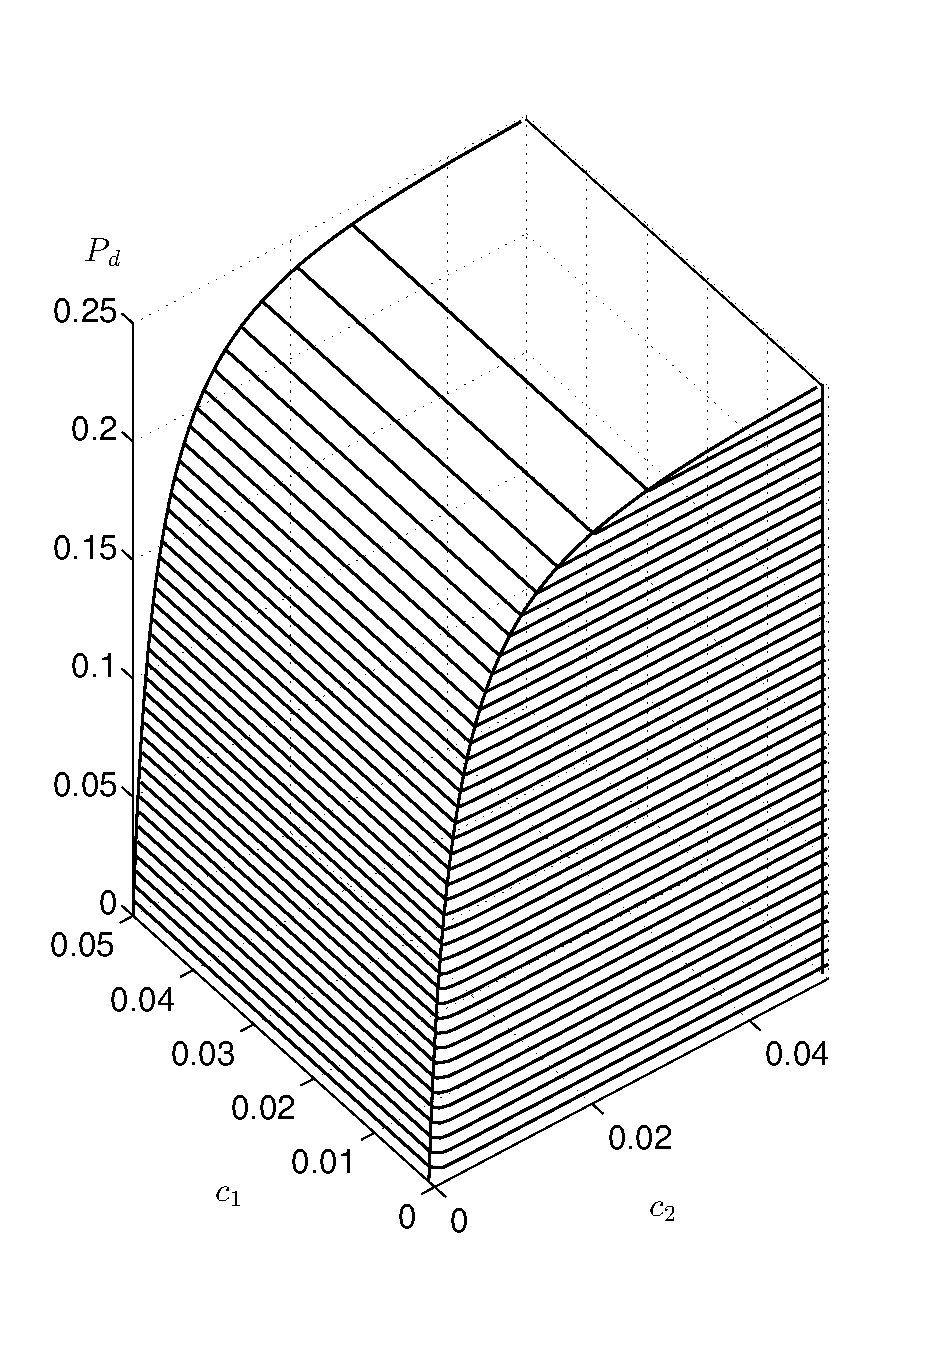
\includegraphics[width=12cm, height=16cm]{4/ROCsurface.eps}
  \caption{M-ROC surface for cyclostationary detector.}
  \label{pic:1221n0}
\end{figure}
